\documentclass[../../main-detail.tex]{subfiles}
\begin{document}

\chapter{形式文法}
\begin{leftwavybox}
\textbf{章全体の完成度（5段階，5が最高）}：誤りの少なさ2，文章の簡潔さ3，話題の網羅性3．
論点は広く揃っているが，前方照応，一般の線形化に未確定部分が残る．
\end{leftwavybox}
\section{はじめに}
\begin{leftwavybox}
\textbf{完成度（5段階，5が最高）}：誤りの少なさ 4，文章の簡潔さ 3，話題の網羅性 2．
目的と構成は明確だが，集合論と型理論の比較が未完である．
\end{leftwavybox}
% この章では\textbf{文語コノメノ}(胡：keltokono)を扱う．文語については，以下の点が主なテーマになる．
述語論理等で定式化される既存（あるいは独自）の意味論および形式存在論の枠組みをコノメノで厳密に議論するために，形式文法を導入する．具体的には以下が論点になる：
\begin{enumerate}
    % \item （形式文法に限らない）コノメノの基本的な文法観と特徴を整理する．
    \item さまざまな意味論が同じ文法のインターフェイスの下で衝突を起こさずに統一的に扱えるのかを，実際に体系を定義して検証する．
    \item 口語において話者の直感や良心に任されていた曖昧な文法規則を，形式言語としてどのように違和感なく定式化できるかを探る．（現版では，線形文モジュールが主な対象である．）
\end{enumerate}
進め方としては，（形式文法に限らない）コノメノの基本的な文法観と特徴を整理した上で，単純な体系から始めて段階的に文法を拡張し，自然言語に近い実用的な方へと進める．本章の構成は，論理コアである\textbf{基本体系}の上に，表層の\textbf{モジュール}（グラフ，線形文，指示詞，談話等）を載せる形をとる．
\begin{remark}
    従来の呼称「体系P」「体系S」「体系D」は，それぞれ基本体系，線形文モジュール，談話モジュールを指す．
\end{remark}
将来の展望としては以下のようなことを考えている（コノメノの既存文法を修正することは高コストであるため，一部は別の言語として実装する可能性が高い）：
\begin{enumerate}
    \item 意味論だけでなく証明論も定義し，健全性・完全性およびオントロジーとの整合性を検証する．
    \item 本章で定義する形式文法を Lean で書き直す．それとともに，コノメノをプログラミング言語として実装し，自動証明や意味処理への応用を目指す．（\cite{auto-prover}(旧)，\cite{formalization}(新)等のリポジトリで部分的に実装されているが，現在 pending の状態である．）
\end{enumerate}

\subsection{文法観と特徴}\label{sec:grammar-view}
\paragraph{平坦性とKG}\label{par:flat-kg}
コノメノの特徴として語られていた性質に「平坦性」がある．一般に，文や句，節といった言語表現は，2分木の構造を持つとして説明される．しかし，単純に，物事の性質や関係性あるいはイベントの発生等について情報を与えるある種の文については，語彙レベルの基本的な関係を連言で繋げていくことのみで表現できる．例えば，「青い球が机の上で転がる」という文を考えると，「球が青い」「球が机の上にある」「球が転がる」という3つの関係を連言で繋げて表現することができる．このような表現方法は，\textbf{知識グラフ}(Knowledge Graph, KG)の考え方にも近く，グラフ表現を導入する自然な理由の1つになる．

後述のグラフ表示（\S\ref{sec:graph-notation}）はこの見方を文字どおり構文化する．平坦な関係連言にとって自然な表示はグラフであり，交互型線形文は，そのグラフを発話・筆記の1次元上へ無理に射影した表示である．

しかし，すぐわかるようにこのような表現方法には限界がある：量化や連言以外の論理演算（否定・選言など）ができない．これに関しては（妥協策として），述語論理の原子命題にあたる位置に，何らかの形でKGを埋め込み，1階論理と統合することになった．

\paragraph{束縛変数の埋め込み} 自然言語では，量化子がその束縛変数の動く範囲を修飾するように文中に埋め込まれている．例えば，「机の上の\emph{全ての}紙に\emph{何らかの}名前が書かれている」という文を考える．これを述語論理的に書けば，「$\forall x \in \text{机の上の紙}.\; \exists y \in \text{名前}.\; y\ \text{は}\ x\ \text{に書かれている}$」となる．このように，述語論理では明示的に変数記号を導入し，量化子と束縛変数の動く範囲をもとの文の外側まで動かすのだが，自然言語ではもとの文に埋め込んで表現する．コノメノでは，後者の束縛変数の埋め込みを採用し，束縛変数の動かす範囲を「第1スコープ」，もとの文を「第2スコープ」と呼ぶ．

コノメノでは，束縛変数を取る語彙を総称して\textbf{冠詞}と呼ぶ\suppl{機能に即した「パラメタ演算子」のような名も考えられるが，見た目と親しみやすさから冠詞と呼ぶ}．冠詞は$\forall$や$\exists$といった典型的な量化子以外に，「ほとんどの$A$」「少なくとも3つの$A$」といった一般化量化子，内包的な集合構成（関係節の文脈で登場する），疑問符や引用符など，さまざまな役割を統合する枠組みである．

\iffalse
\paragraph{集合論 vs 型理論} 数学を形式化する基礎論には集合論と型理論がある．前者は，数学の標準的な世界観であり，1階述語論理(FOL)の上に公理系を設定することで構築され，後者は，証明支援系の世界観であり，Martin-Löf型理論やCalculus of Inductive Constructions (CIC)のような強力な依存型の体系が用いられる．

% そして，...%\cite{hol-web, hol-book}などの単純型で型付けされた高階論理(HOL)は，集合$X$から始めて任意有限回の冪で到達できる集合$R_\omega(X)$と大まかに対応する．形式意味論の標準的な枠組みは HOL と相性が良いが，やはりそれだけでは可能な操作が少なく，型を潰す操作を入れて部分的に型無しにしてしまう（集合論寄り）か，型を強化して表現力を上げる（型理論寄り）かという選択が生まれる．コノメノは前者を採用している．

\todo{
% 型理論寄りの意味論（Heim--Kratzer）や property theory，圏論的意味論を採らない理由（数の扱いなど）をここで議論する．
\begin{enumerate}
    \item Heim \& Kratzer 等の教科書的な意味論は，単純型付きラムダ計算を基礎にしている $\to$ 数やその演算は書ける？「ここに3人いる，あそこに2人いる．$\to$こことあそこに5人以下いる(注：共通領域があるかもしれないので$\leq 5$)」
    \item Leanでも数や部分集合の扱い方がめんどくさかった気がする．
    \item 集合論が一番使い勝手がいい．できるだけ1階で済ませるようにする．
\end{enumerate}
ここから埋め込みの話(意味論章寄り)
\begin{enumerate}
    \item 表現の埋め込みと集合の埋め込みがある．前者は冠詞，後者は名詞化子(専用の機構)で扱う．意味論章のTarski, Russellに対応．
    \item 自己言及をしっかり扱うなら，終余代数的なやり方がいい．$\to$ 今後の展望として圏論的意味論に移る
    \item property theory (特にFrege structure？)もここら辺の話？
\end{enumerate}
表現の埋め込み$\to$超内包性．疑問などを含む．
\todo{オントロジー側の機構である種概念が高階の問題にも超内包性の問題にも対応する万能な考え方かもしれない．}
}
\fi



\section{辞書}
\begin{leftwavybox}
\textbf{完成度（5段階，5が最高）}：誤りの少なさ 3，文章の簡潔さ 4，話題の網羅性 4．
語彙の型とソート制約は定まっているが，実装済み辞書との全体照合は未完である．
\end{leftwavybox}
まずは，辞書と語彙(述語論理でいう``言語'')を導入する．実際の辞書とは整理の仕方が一部違うことに注意．辞書も体系ごとに拡張されていく．

\begin{definition}[型]
    型$T$は，真理値の型$\Omega$と個体の型$V$からはじめて，関数と直積を組み合わせたものである：
    $$
        T ::= 1 \mid \Omega \mid V \mid T \to T \mid T \rightharpoonup T \mid T \times T
    $$
    また，curryingとun-curryingができるものとする：
    \begin{align*}
        (\alpha \times \beta) \to \gamma \;&\simeq\; \alpha \to (\beta \to \gamma)
    \end{align*}
    1は単位型であり，$\alpha \times 1 \simeq \alpha$や$\alpha^1 \simeq \alpha,\; 1^\alpha \simeq 1$などが成り立つものとする．
\end{definition}
\begin{remark}
    ここで$V$は個体の型であり，その解釈領域には集合だけでなく原子も含める（後述の解釈領域の定義）．
\end{remark}
\begin{definition}[辞書]\textbf{辞書}は，以下のデータからなる：
    \begin{itemize}
        \item $L$：語彙の集合．$a\in L$に対して，$\arity a \in \mathbb{N},\; \isFunc a \in \{0, 1\}$が定義される．$\arity a$は$a$のアリティを表し，$\isFunc a$は$a$が関数であるかどうかを表す．
        \begin{align*}
        \begin{array}{ccccc}
            \toprule
            \isFunc \setminus \arity & 0 & 1 & 2 & \cdots \\
            \midrule
            0 & \text{命題定数} & \text{1項述語} & \text{2項述語} & \cdots \\
            1 & \text{定数} & \text{1項関数} & \text{2項関数} & \cdots\\
            \bottomrule
        \end{array}
        \end{align*}
        \begin{itemize}
            \item $\tArity a = \arity a + \isFunc a$とする．
            \item $A_n = \{a \in L \mid \tArity a = n\}$とする．特に$A = A_1$は概念の集合と呼ばれる．
            \item $R_n = \{a \in L \mid \arity a = n, \isFunc a = 0\}$を$n$項述語の集合と呼ぶ．
            \item $F_n = \{a \in L \mid \arity a = n, \isFunc a = 1\}$を$n$項関数の集合と呼ぶ．
            \item $\dom a \in A^{\tArity a}$が定義される．$\dom a$は，$a$の引数の定義域（と関数であれば値域）を表す．
            \item $\type a$は，$a$の型を表す．$\isFunc a = 0$のとき，$\type a = V^{\arity a} \to \Omega$であり，$\isFunc a = 1$かつ$\arity a>0$のとき，$\type a = V^{\arity a} \rightharpoonup V$であり，定数$a\in F_0$の型は$V$である．
        \end{itemize}
        \newcommand{\cod}{\mathop{\mathrm{cod}}}
        \item $Q$：冠詞の集合．各冠詞$q\in Q$には\textbf{冠詞署名}$\langle\mathrm{arg}\,q,\ \mathrm{keep}\,q,\ \mathrm{out}\,q\rangle$が定義される：
        \begin{itemize}
            \item $\mathrm{arg}\,q\in\{\Omega, V\}$：（変換前の）第2スコープの入力型．式を取る冠詞は$\Omega$，項を取る冠詞は$V$．
            \item $\mathrm{keep}\,q\in\{1, V\}$：第1スコープの割り当てを，冠詞固有の方法で集約して結果の添字に残さない（$\mathrm{keep}\,q=1$）か，添字として保持する（$\mathrm{keep}\,q=V$）か．
            \item $\mathrm{out}\,q\in\{1, V\}$：各添字に対して返す値を，真理値$\Omega^1\simeq\Omega$（$\mathrm{out}\,q = 1$）とするか，クラス$\Omega^V$（$\mathrm{out}\,q = V$）とするかを表す出力標識．\textbf{個体$V$を直接返す冠詞は許さない．}
        \end{itemize}
        $\alpha,\beta\in\{1,V\}$，$\gamma\in\{\Omega,V\}$に対して
        \[
            Q^{\gamma}_{\alpha,\beta} = \{q\in Q \mid \mathrm{arg}\,q=\gamma,\ \mathrm{keep}\,q=\alpha,\ \mathrm{out}\,q=\beta\},\qquad
            Q_{\alpha,\beta} = \bigcup_{\gamma\in\{\Omega,V\}} Q^\gamma_{\alpha,\beta}
        \]
        とする．署名から\textbf{適用結果型}（(Plm-pt)が与える型）が決まる：有限ラベル列$I$に対して
        \[
            \mathrm{Result}(I;\alpha,\beta) := \alpha^I\to\Omega^\beta
            \simeq (\alpha^I\times\beta)\to\Omega.
        \]
        少なくとも以下の種類の冠詞が必要である：
        \begin{itemize}
            \item $Q_{1,1}$：量化子．少なくとも$\forall, \exists$が含まれ，$\mathrm{Most}, \mathrm{Many}$，および$[K], \langle K\rangle$（形式意味論章）もここに入る．$\mathrm{Ind}$（口語\ko{anic}「不特定の」）は独立の冠詞とせず，内包動詞の内容対象位置における$\exists$の糖衣とみる（形式意味論章「内容対象方式」．de dicto冠詞$N$を採らないのと同じ理由）．\memo{\ko{anic}が糖衣で尽くせるか（内包動詞以外での不特定読み）は未検証．}
            \item $Q_{V,1}$：内包化演算子．$L, F$．割り当てを保持して各割り当てに真理値を返す，すなわち充足する割り当てのクラス（$V^I\to\Omega$）を作る．$L$は内包化，$F$は文脈内包化と呼ばれる．
            \item $Q_{1,V}$：証拠演算子．$C, E, K$．$C$は文を成立させる状況のクラス，$E$はその選択肢（情報状態のクラス），$K$は成立する世界のクラスを作る（形式意味論章）．
            \item $Q_{V,V}$：族版演算子．割り当てごとにクラスを返す（$V^I\to\Omega^V$）．$M$（引用符），$\mathrm{Cf}, \mathrm{Kf}$（形式意味論章），および$\mathrm{Lf}$（ラムダ抽象．$\mathrm{arg}\,\mathrm{Lf}=V$）．$M$と$\mathrm{Lf}$の非空の切片は単元クラスである（関数性）．
        \end{itemize}
        現時点で$\mathrm{arg}\,q = V$の冠詞は$\mathrm{Lf}$であるが，項を取る冠詞は今後増えうる．
        \item $X$：変数全体の集合．コノメノにおいては変数は便宜的なもので，解釈途中以外には現れない．
    \end{itemize}
    各$A_n$に対して，概念の上位-下位関係を表す順序関係$\preceq$が定義される．これは$\dom_i$と両立する(言い換えれば$\dom_i$が単調である)とする．すなわち，$a \preceq b$であるとき，任意の$i$について$\dom_i a \preceq \dom_i b$が成り立つ．
\end{definition}
\begin{definition}[ラベル集合]
    辞書には含まれないが，添字をつけるためのラベル集合が必要である．ラベル集合$\Lambda$は，濃度が可算無限以上であればなんでも良いが，基本的には自然数全体の集合とする．(なお，口語では，ラベル相当のものを活用で表現するため，ラベル集合は現れない．)
\end{definition}

\section{基本体系}
\begin{leftwavybox}
\textbf{完成度（5段階，5が最高）}：誤りの少なさ 2，文章の簡潔さ 3，話題の網羅性 3．
部分項の形成と評価は定まっているが，複合的な適用例の検算を増やす必要がある．
\end{leftwavybox}
\subsection{1階述語論理(FOL)の復習}
比較のために，1階述語論理の文法を定義しておこう．述語論理の辞書は，$Q = \{\forall, \exists\}$のみである．また，$L,Q$以外に変数全体の集合$X$を持つ．
\begin{definition}[FOLの文法]
    以下のような規則で型$\alpha$の表現$\mathrm{Rep}(\alpha)$を帰納的に定義する．FOLで意味を持つ型は，語彙 $L$ を別にすれば，$V$（項）と$\Omega$（式）だけである．
    \[
    \infer[\text{(Var)}]{
        x: V
    }{
        x \in X
    }
    \]
    \[
    \infer[\text{(Func-App)}]{
        f(t_1, \cdots, t_n): V
    }{
        t_i : V\; (i=1,\cdots,n),\quad f \in F_n
    }
    \]
    \[
    \infer[\text{(Pred-App)}]{
        P(t_1, \cdots, t_n): \Omega
    }{
        t_i : V\; (i=1,\cdots,n),\quad P \in R_n
    }
    \]
    \[
    \infer[\text{(Quant)}]{
         q x.\phi: \Omega
    }{
         x\in X,\quad q\in Q,\quad \phi: \Omega
    }
    \]
    \[
    \infer[\text{(Logic-1)}]{
         \lnot\phi: \Omega
    }{
         \phi: \Omega
    } 
    \qquad
    \infer[\text{(Logic-2)}]{
         \phi \mathbin{@} \psi: \Omega
    }{
         \phi: \Omega,\quad  \psi: \Omega,\quad @\in \{\land, \lor, \to, \cdots\}
    }
    \]
\end{definition}
\subsection{構文}
述語論理に，量化子の埋め込み・一般化を導入した文法を定義する．コノメノの意味論は基本体系の冠詞の扱いに集約される．
\todo{overviewで先行研究調べたのでそれと比較すると良いかも．}
実際の会話では線形文モジュールが主に使われるが，意味論の議論のためには基本体系で十分である．
この体系は，FOLと高階論理(\cite{hol-web, hol-book}など)の中間のような文法を持っている．
\begin{definition}[体系Pの文法]
    以下のような規則で型$\alpha$の表現$\mathrm{Rep}(\alpha)$を帰納的に定義する．
    \[
    \infer[\text{(Voc)}]{
        a: \type a
    }{
        a \in L
    }
    \qquad
    \infer[\text{(Var)}]{
        x: V
    }{
        x \in X
    }
    \]
    \[
    \infer[\text{(App)}]{
        f(t): \beta
    }{
        t: \alpha,\quad f: \alpha\to \beta
    }
    \qquad
    \infer[\text{(Concat)}]{
        t\circ s : \alpha \times \beta
    }{
        t: \alpha,\quad  s: \beta
    }
    \]
    \[
    \infer[\text{(App-p)}]{f(t):\beta}{t:\alpha,\quad f:\alpha\rightharpoonup\beta}
    \]
    \[
    \infer[\text{(Plm-at)}]{
         t^{d_i}: V
    }{
         t: V \to \Omega,\quad d\in Q,\quad i\in \Lambda
    }
    \]
    \[
    \infer[\text{(Plm-pt)}]{
         \{u\; d_{i_1, \cdots, i_n}\}: \mathrm{Result}(I;\mathrm{keep}\,d,\mathrm{out}\,d)
    }{
         u: \mathrm{arg}\,d,\quad d\in Q,\quad I=(i_1, \cdots, i_n)\ \text{は相異なるラベルの列}
    }
    \]
    ここで，添字$i_1, \cdots, i_n$は，$u$の中に実際に現れる接辞付き項$t^{d_{i_k}}$（各$k$）との対応関係を示すラベルである．すなわち，$\{u\; d_{i_1,\cdots,i_n}\}$は，$u$内でラベル$i_1,\ldots,i_n$のいずれかを持つ接辞付き項を$d$によって束縛することを意味する（詳細は量化の対応関係の探索を参照）．
    % 結論の型は冠詞署名から$\mathrm{Result}$で決まる：$\mathrm{keep}\,d=1$なら$\Omega^{\mathrm{out}\,d}$（例：$\forall$なら$\Omega$，$C$なら$\Omega^V$），$\mathrm{keep}\,d=V$なら割り当て$V^I$から$\Omega^{\mathrm{out}\,d}$への関数型（例：$L$なら$V^I\to\Omega$，$M$なら$V^I\to\Omega^V$）．$I=\emptyset$なら後者も$\Omega^{\mathrm{out}\,d}$とみなす．
    % 割り当てを保持する冠詞の結果は全割り当て上の関数として表し，第1スコープ$S$の外では結果型の底値（$\Omega$なら偽，$\Omega^V$なら空クラス）を返す．% ←どゆこと
    部分演算の項は次の規則で形成する．
    \[
    \infer[\text{(Nom)}]{\setop P:V}{P:V\to\Omega}
    \quad
    \infer[\text{(Cls)}]{\clsop t:V\to\Omega}{t:V}
    \quad
    \infer[\text{(The)}]{\mathrm{the}(P):V}{P:V\to\Omega}
    \]
    \[
    \infer[\text{(Set-App)}]{\mathrm{apply}(f,t):V}{f:V,\quad t:V}
    \]
    多成分の割り当てのクラスには，後述の組個体上の述語への変換を先に施す．
    $M$・$\mathrm{Lf}$のように各切片が単元クラスである冠詞については，切片の唯一の要素を返す部分演算$\mathrm{the}(\bullet)$を認める．
    \memo{$\mathrm{the}$の口語がない．}
    \[
    \infer[\text{(Stl)}]{
        t_1\; r_1\; t_2\; r_2\; \cdots\; r_{n-1}\; t_n: \Omega
    }{
        t_i: V\quad r_j: V \text{ or } r_j \in R_2
    }
    \]
    \[
    \infer[\text{(Logic-1)}]{
         \lnot\phi: \Omega
    }{
         \phi: \Omega
    }
    \qquad
    \infer[\text{(Logic-2)}]{
         \phi \mathbin{@} \psi: \Omega
    }{
         \phi: \Omega,\quad  \psi: \Omega,\quad @\in \{\land, \lor, \to, \cdots\}
    }
    \]
    加えて，以下のような略記を許す．
    \begin{itemize}
        \item $f(t_1,t_2,\cdots,t_k)$は，$[t_1\; f\; t_2\; \cdots\; t_k]$と書いても良い(というより通常はこのように書く)．$k$は$\arity f$と等しい必要はなく，$t_i : V^{n_i}$のとき，$\sum_{i=1}^k n_i = \arity f$であれば良い．
        \item $Q$のラベルは対応が明確であれば省略しても良い．$\{\phi(t^{d}, t^{d})\; d\}$のように，ラベル無しの項が複数現れる場合は，$\{\phi(t^{d_i}, t^{d_j})\; d_{ij}\}$のように異なるラベルを持つものとして解釈する．
        \item $\land$は$,$と書いても良い．
        \item 文の1番外側の(Plm-pt)は明確であるから省略しても良い．
        \item $\{\{\phi\; d_{I}\}d_{J}\}$のように連続したPlm-ptは，括弧を省略して$\{\phi\; d_{I}d_{J}\}$と書いても良い．
    \end{itemize}
\end{definition}
\subsection{解釈}
\begin{definition}[解釈領域]
    個体型$V$の解釈領域を$\mathcal{M}$と書く．原子の集合$U$と正則な非可算基数$\kappa$を固定し，
\[
    \mathcal{M} = H_\kappa(U) = \{x \mid \text{$x$は$U$上の集合であり，推移閉包の濃度が$\kappa$未満}\} \cup U
\]
とする．型$T$に対する解釈領域$D(T)$を，以下のように定義する．
\begin{itemize}
    \item $D(1)=\{*\}$（単位型）．
    \item $D(V) = \mathcal{M}$．
    \item $D(\Omega) = 2 = \{0, 1\}$．
    \item $D(\alpha \to \beta) = \mb{D(\alpha), D(\beta)}$．
    %ここで，$[X, Y]$は，$X$から$Y$への関数全体の集合を表す．
    \item $D(\alpha \times \beta) = D(\alpha) \times D(\beta)$．
    \item $D(\alpha\rightharpoonup\beta)$は$D(\alpha)$から$D(\beta)$への部分関数全体．
\end{itemize}
\end{definition}
\begin{remark}[解釈領域に求める閉包性]
    $\kappa$の正則性により，$A\subseteq\mathcal{M}$かつ$|A|<\kappa$なら$A\in\mathcal{M}$となる：$A$の要素の推移閉包を$\kappa$未満個集めても，その和の濃度は$\kappa$未満である．これにより，有限タプルや小さいクラスの名詞化を領域内で扱える．非可算性は，可算段階の構成にもこの閉包性を使うために置く（辞書章のchaseなど）．これは全個体について冪集合の個体化を要求することとは異なる．
    \memo{2026-09-08：言語の基本意味論に必要な閉包性と，数学を扱うための追加要件を分けて精査する．現行の正則非可算性を基本条件とし，解釈領域の純粋集合部分にZFC全体を要求するかは未決とする．ZFCの公理を翻訳できることだけでは，それらをこの領域で真とする要求にはならない．}
\end{remark}
\begin{whynot}
    解釈領域を有限ランクの集合（$\mathcal{M} \supseteq R_\omega(U)$）で構成する案は採らない：$R_\omega(U)$は有限タプルには閉じているが，小さい部分集合を取る操作には閉じていない．例えば，ランクが有界でない可算個の要素を集めた集合は有限ランクに収まらない．型を潰す操作を多用する本言語では，「小さい集合はすべて個体である」という$H_\kappa$型の閉包の方が摩擦が少ない．なお$H_\kappa(U)$のもとでも$\mb{M,2}$（クラス全体）や$\mb{M,M}$は$M$の外にあり，これは名詞化子の部分性（\ref{subsec:nominalizer}節）として言語側に現れる．
\end{whynot}
\begin{remark}
    有限変数割り当ての全体について$\mathrm{Fin}(X, \mathcal{M}) \subseteq \mathcal{M}$が成り立つ（変数名を$\mathcal M$内へ符号化しておけば，有限なグラフも遺伝的に小さい）．したがって第1スコープ$S \subseteq \mathrm{Fin}(X,\mathcal{M})$の\emph{要素}は常に個体であり，$S$\emph{自身}は$|S| < \kappa$のときに限り個体である．$S$は量化のドメインとしてメタレベルで使われるだけなので，$S$自身が個体である必要はない．ただしこの保証は「第1スコープに現れる項の解釈が$M$の部分クラスであること」に依存しており，これを体系の不変条件とする．
\end{remark}
\iffalse
\begin{remark}
    後述する具体的な演算子を考えると，$\mathcal{M}$は統語的な表現を記号として埋め込む関数$\iota : \bigcup_{\alpha} \mathrm{Rep}(\alpha) \to \mathcal{M}$を少なくとも1つ（始域は構文表現のみ．意味値やクラス全体の個体化は要求しない）\footnote{表現$\phi$に対して，「文字列$\phi$」「命題$\phi$」...など複数の埋め込みがあり得る．}持っている必要があるだろう．
\end{remark}
% ↑冠詞Mの変種 + the で対応できる
\fi
\begin{definition}[変数割り当て関数]
    (全域/部分/有限)変数割り当て関数$\sigma$はそれぞれ，$X$から$\mathcal{M}$への(写像/部分写像/有限部分写像)である．
\end{definition}
\begin{definition}[語彙割り当て関数]
    (全域/部分/有限)語彙割り当て関数$\rho$はそれぞれ，$L \cup Q$から$\bigcup_{\alpha} D(\alpha)$への(写像/部分写像/有限部分写像)である．これは以下の条件を満たすものとする．
    \begin{itemize}
        \item $a\in L$の値は$D(\type a)$に属する．$B_i=\widetilde\rho(\dom_i a)$とし，$\widetilde\rho(B)$は概念ならその外延，定数なら値の単元集合とする．
        \begin{itemize}
            \item $a\in R_n$：真になる引数列の集合は$\prod_{i=1}^n B_i$に含まれる．
            \item $a\in F_n$，$n>0$：$\rho(a)$の定義域は$\prod_{i=1}^n B_i$で，値は$B_{n+1}$に属する．ソート外の入力では未定義となる．
            \item $a\in F_0$：$\rho(a)\in B_1$．
        \end{itemize}
        \item 冠詞$d\in Q$，各有限ラベル集合$I$，外側の変数環境$\sigma$に対して，\textbf{冠詞解釈型}$\rho_{I,\sigma}(d) \in \mb{\wp(\mathcal{M}^I) \times \mathrm{Rep}(\mathrm{arg}\,d),\; D(\mathrm{Result}(I;\mathrm{keep}\,d,\mathrm{out}\,d))}$．$\mathcal{M}^I$は$I$から$\mathcal{M}$への割り当て全体(第1スコープに当たる)，$\mathrm{Rep}(\alpha)$は型$\alpha$を持つ表現全体の集合である(第2スコープに当たる)．
    \end{itemize}
\end{definition}
\begin{remark}
    以下では$I$と外側の環境$\sigma$が明らかなとき，$\rho_{I,\sigma}(d)$を$\rho(d)$と略記する．内側の式は，冠詞の規則に従って環境を更新して評価する．\textbf{$Q$の解釈は外延のみで決まらない}：第2スコープは意味値ではなく表現として渡し，同じ意味値を持つ表現が同じ結果を与えるとは仮定しない．
\end{remark}

$I$はラベルの列とする．$\{\phi d_I\}$という形式の文について，量化子$d_I$に束縛される接辞付き項$t^{d_i}$を探索したい．これは構文木の走査$+$シンボルテーブルで実装できる．
\begin{definition}[量化の対応関係の探索]
    環境を表すスタック$E$と，結果を格納するマップ$R$，変数との対応関係を格納するマップ$U$を用意し，文の構文木を深さ優先探索(前順走査)する．このとき，
    \begin{itemize}
        \item $\{\phi d_I\}$の形式の文を見つけたら，
        \begin{enumerate}[label=(\arabic*)]
            \item $d_I$ (正確にはその位置のポインタ) を$E$にpushし，$R[d_I] = []$と初期化する．
            \item 子ノード$\phi$を再帰的に探索する．
            \item $E$から$d_I$をpopする．
        \end{enumerate}
        \item 接辞付き項$t^{d_i}$を見つけたら，スタックの要素$p_I\in E$を上から順に見ていき，$p = d,\; i\in I$となるものを見つけたら，$R[p_I] \leftarrow R[p_I] \circ [t^{d_i}]$と更新する(正確にはその位置のポインタを格納する)．
    \end{itemize}
\end{definition}
\begin{definition}[スコープの決定]
    $\{\phi d_I\}$について，上の量化の対応関係の探索によって得られるマップ$R$を用いて，$T = R[d_I]$（$d_I$に束縛される接辞付き項の一覧）とする．このとき，$t^{d_i}, {t'}^{d_j}\in T$に対して，
    \begin{align*}
        t^{d_i} \sim {t'}^{d_j} \iff i = j
    \end{align*}
    という同値関係を定義する．このとき，$d_I$の(第1)スコープは，
    \[
       S = \prod_{C \in T/{\sim}} \bigcap_{t \in C}\lbb t\rbb\quad  (\subseteq \mathcal{M}^n)
    \]
    である．ここで直積は，
    \[
    \prod_{\lambda\in \Lambda} X_\lambda = \Bigl\{f:\Lambda \to \bigcup_{\lambda\in \Lambda} X_\lambda \mid \forall \lambda\in \Lambda.\; f(\lambda) \in X_\lambda\Bigr\}
    \]
    のように関数で表示される場合と，$|\Lambda| < \infty$のときには順序対の集合として表示される場合がある．基本的に前者を採用するが，後者の場合を採用することもある．その場合，$T/{\sim}$の要素を1列に並べる必要があるが，それは$[t^{d_i}] \leq [{t'}^{d_j}] \iff i \leq j$のように定める．
\end{definition}

\begin{definition}[変数への置き換え]
    項の同値類を変数で置き換える単射$\iota : T/{\sim} \hookrightarrow X$を用意し，文中の接辞付き項$t^{d_i}$を$\iota([t^{d_i}])$で置き換える．$[t^{d_i}]\in T/{\sim}$をそのまま使っても良いが，これは変数割り当て$\sigma$の始域を簡潔にするための措置である．場合によっては，$[t^{d_i}]$と$\iota([t^{d_i}])$を同一視しても良い．像の変数は外側の自由変数および他の束縛に使う変数と異なるものを選ぶ．各同値類をそのラベル$i\in I$に対応させ，$a:I\to\mathcal M$を$\iota([t^{d_i}])\mapsto a(i)$へ移す．この対応により，$S$の要素を有限変数割り当てとして扱う．
\end{definition}

\begin{definition}[全体の解釈]
    解釈関数$\lbb \bullet \rbb_{\rho,\sigma}$は，以下のように定義される．解釈関数は，上で述べた語彙割り当て関数$\rho$と，変数割り当て関数$\sigma$に依存するが，明確であれば省略する．
    \begin{itemize}
        \item $\lbb f(t) \rbb = \lbb f \rbb(\lbb t \rbb)$．
        \item $\lbb t \circ s \rbb = \lbb t \rbb \circ \lbb s \rbb$．
        \item $\lbb \{\phi d_I\} \rbb_{\rho,\sigma} = \rho_{I,\sigma}(d)(S, \phi)$．
        \item $\lbb x \rbb = \sigma(x)\;\; x:\text{変数}$．項で書くと$\lbb t^{d_i} \rbb = \sigma([t^{d_i}])$．
        %$t^{d_i}$が何らかの冠詞によって束縛されている場合，$t^{d_i}$は変数で置き換えられるため，単体で解釈されることはない．そのような束縛がないとき（通常は，$d$が$F$であるとき）は，$\sigma$(変数割り当て)によって解釈を付与する．
        \item $\lbb t_1\; r_1\; \cdots\; r_{n-1}\; t_n \rbb = 1 \iff \forall i\in \{1,\ldots,n-1\},\; \langle \lbb t_i\rbb, \lbb t_{i+1}\rbb\rangle \in \lbb r_i \rbb$．
        \item $\lbb \lnot \phi \rbb = \lnot \lbb \phi \rbb$．
        \item $\lbb \phi \mathbin{@} \psi \rbb = \lbb \phi \rbb \mathbin{@} \lbb \psi \rbb$．
    \end{itemize}
    % なお，変数割り当て関数は，$t^{d_i}$という形の項（形が同じでも位置によって区別する）に対して$M$の要素を割り当てる部分関数である．
\end{definition}
\begin{definition}[未定義の伝播]\label{def:undefined-propagation}
    $\lbb t\rbb\uparrow$は項$t$の値が定義されないことを表す．$\uparrow$を個体や対象言語の定数として追加しない．式の形成可能性と，その値の定義可能性を区別する．
    \begin{itemize}
        \item 関数適用は，関数または引数が未定義，あるいは引数が部分関数の定義域外なら未定義となる．ただし述語適用（結果型$\Omega$）では偽とする．
        \item 直積の成分，順序組の成分，名詞化・述語化・$\mathrm{the}$・集合による関数適用の引数に未定義があれば，その結果も未定義となる．$\mathrm{the}$は単元クラスでない場合にも未定義となる．
        \item 未定義項を含む原子式は偽とする．否定・連言などの論理演算は，この2値の結果へ通常どおり適用する．したがって未定義項を含む原子式の否定は真になりうる．
        \item 第1スコープの述語が未定義なら，その外延を空としてスコープを作る．量化は$\mathcal M$内の定義された個体だけを動かす．
        \item 冠詞の第2スコープは構文のまま渡す．$M$は未定義項を含む式も引用でき，$\mathrm{Lf}$は値が未定義の切片を空クラスにする．
    \end{itemize}
\end{definition}
\begin{example}
    後者関数$s$の入力ソートが自然数なら，$s(\ko{meacc}^{F_1})$はその値が猫である割り当てのもとで未定義となる．さらに関数を適用しても未定義が伝播し，それを含む等式は偽になる．名詞化不能なクラス$P$から作った$f(\setop P)$も同じ規則に従う．
\end{example}
\begin{remark}[第1スコープ・第2スコープの対応]
    §\ref{sec:grammar-view}で導入した「第1スコープ」「第2スコープ」と定義の対応を整理する．
    \begin{itemize}
        \item \textbf{構文側}：接辞付き項$t^{d_i}$が第1スコープ（束縛変数の動く範囲を表す述語），$\{\phi\; d_I\}$中の式本体$\phi$が第2スコープに相当する．
        \item \textbf{意味側}：$\lbb\{\phi\; d_I\}\rbb = \rho(d)(S, \phi)$において，$S$（第1スコープの解釈，量化の域）と$\phi$（第2スコープ）が対応する．
    \end{itemize}
\end{remark}

\subsection{冠詞の具体例}
\noindent
具体的に，$d\in Q$のいくつかの例をみていこう．それ以外にも，実際に運用するにはいくつか特殊な定数が必要である．
\begin{definition}
    $\forall, \exists$は，文字通り全称量化子と存在量化子であり，$L$は内包的に集合を作る演算子である．%，$E$はinquisitive semanticsの構成によって疑問文を作る演算子である．

    文$\phi$と変数割り当て$\sigma$に対して，$\phi(\sigma)$は$\phi$にある$\dom \sigma$の項を$\sigma$によって置き換えたものとする．また，$\sigma, \sigma'$が変数割り当てのとき，$\sigma\vll\sigma'$は，$\sigma$を$\sigma'$に更新した変数割り当てである．つまり，
    \begin{align*}
    (\sigma\vll\sigma')(x) = \sigma'(x) \text{ if } x \in \mathrm{dom}(\sigma') \text{ else } \sigma(x)
    \end{align*}
    ここで，
    $\lbb \phi(\sigma')\rbb_{\rho,\sigma} = \lbb \phi\rbb_{\rho, \sigma\vll\sigma'}$である．このような定義のもとで，$\forall, \exists, L$などの解釈は以下のようになる．
    \begin{itemize}
        \item $\forall \in Q^\Omega_{1,1}$．$\rho(\forall)(S, \phi) = (\forall \sigma' \in S.\; \lbb \phi\rbb_{\rho, \sigma\vll\sigma'} = 1)$．
        \item $\exists \in Q^\Omega_{1,1}$．$\rho(\exists)(S, \phi) = (\exists \sigma' \in S.\; \lbb \phi\rbb_{\rho, \sigma\vll\sigma'} = 1)$．
        \item $L \in Q^\Omega_{V,1}$．$\rho(L)(S, \phi) = \{\sigma' \in S \mid \lbb \phi\rbb_{\rho, \sigma\vll\sigma'} = 1\}$（充足する割り当てのクラス．$V^I\to\Omega$の特性関数として読み，$S$の外では偽）．
        % \item $E \in Q_{\Omega \to (V \to \Omega)}$．$\rho(E)(S, \phi) = \bigcup_{\sigma' \in S} \wp(\{\rho' \mid \lbb \phi\rbb_{\rho',\sigma\vll\sigma'} = 1\})$．
        \item $\mathrm{Lf} \in Q^{V}_{V,V}$（第2スコープは項$t$）．$a\in\mathcal M^I$に対して
        \[
        \rho(\mathrm{Lf})(S,t)(a)=
        \begin{cases}
            \{\lbb t\rbb_{\rho,\sigma\vll a}\} & a\in S\text{ かつ項の値が定義されるとき},\\
            \emptyset & \text{それ以外}
        \end{cases}.
        \]
        非空の切片は単元クラスであり，値は$\mathrm{the}(\cdot)$で取り出す．

    \end{itemize}
本章ではモデル論的に単純な冠詞のみを定義し，複雑な冠詞は形式意味論章に集める．
\end{definition}
\begin{definition} いくつかの語彙を導入する．口語での言い方も併記する．
    \leavevmode
    \begin{itemize}
        \item $\bot \in R_0$．$\rho(\bot) = 0$．\hspace{1em} (bailek)
        \item $\top \in R_0$．$\rho(\top) = 1$．\hspace{1em} (konston)
        \item $\emptyset \in R_1$．$\rho(\emptyset) = \emptyset$．\hspace{1em} (kwilfon)
        \item $A \in R_1$．$\rho(A) = \mathcal{M}$．\hspace{1em} (alkono)
    \end{itemize}
    さらに，次のような関数や関係を導入する．
    \begin{itemize}
        \item 集合Boole演算子：
        \begin{itemize}
            \item $\lbb [A \cap B] \rbb = \lbb A \rbb \cap \lbb B \rbb$．\hspace{1em} (mite)
            \item $\lbb [A \cup B] \rbb = \lbb A \rbb \cup \lbb B \rbb$．\hspace{1em} (miko)
            \item ほかも同様に．
        \end{itemize}
        \item 関係の転置：$\lbb [R\; \mathrm{me}] \rbb = \{\langle y, x\rangle \mid \langle x, y\rangle \in \lbb R \rbb\}$．\hspace{1em} (me)
        \item タプルのコンストラクタ：$\lbb [t_1\; \mathrm{te}\; t_2] \rbb = \langle \lbb t_1 \rbb, \lbb t_2 \rbb \rangle$．\hspace{1em} (te)
        \item 単元集合：$\lbb [t\; \mathrm{sg}] \rbb = \{\lbb t \rbb\}$．\hspace{1em} (ykof)
        \item 集合の所属関係：$\lbb [t_1\; \in\; t_2] \rbb = 1 \iff \lbb t_1 \rbb \in \lbb t_2 \rbb$．\hspace{1em} (litoi)
        \item 集合の包含関係：$\lbb [t_1\; \subseteq\; t_2] \rbb = 1 \iff \lbb t_1 \rbb \subseteq \lbb t_2 \rbb$．\hspace{1em} (skon)
        \item 等号：$\lbb [t_1\; =\; t_2] \rbb = 1 \iff \lbb t_1 \rbb = \lbb t_2 \rbb$．\hspace{1em} (kast)
    \end{itemize}
\end{definition}
\memo{口語併記必要なんかな？}
\begin{remark}[等濃度と数詞]\label{rem:finite-cardinality}
    \ko{laskast}は等濃度を表す2項関係である．旧版5-2「各種関係(その1)」の定義を，数個体と集合個体の区別を保って移す（2026-09-08改訂・暫定）．
    \begin{itemize}
        \item 集合個体$A,B$について，$A\;\ko{laskast}\;B$は$A$と$B$の間に全単射が存在することを表す．
        \item 自然数個体$n$が自然数$k$を表すとき，$n\;\ko{laskast}\;A$と$A\;\ko{laskast}\;n$は，$A$と$\{1,\ldots,k\}$の間に全単射が存在することを表す．$k=0$では空集合とする．
        \item 2つの自然数個体については，表す自然数が等しいことを表す．
    \end{itemize}
    数個体そのものを集合$\{1,\ldots,k\}$と同一視しない．集合どうしの用法は有限集合に限らない．旧版の短縮$n\;\ko{laskast}=\ko{$n$+las}$も引き継ぐ．現行辞書には未登録であり，移行対象とする．
    順序上の位置や集合体の構成員数とは区別する．集合体を数えるには，構成員を集めた集合を引数に渡す．
\end{remark}
\begin{remark}[単元集合は略記である]
    $\mathrm{sg}$は原始語彙ではなく，$\setop{\{y \mid y\; =\; t\}}$，すなわち$L$と$\mathrm{kast}$と名詞化子の合成の略記である（名詞化子は\ref{subsec:nominalizer}節）．$M = H_\kappa(U)$は個体の単元集合を常に含むので，名詞化子の部分性はこの合成では発火せず，$\mathrm{sg}$は$M$上の全域関数になる．口語形\ko{+ykof}を立てるのは，$x$と$\{x\}$を同一視しない現行の規約のもとで，$\cup$や$\in$の項を作る操作が毎回$L$の括弧を要求するのを避けるためである．
\end{remark}

% あと対象言語型があるのか
\paragraph{$F$の解釈} $\forall$や$L$などの通常の冠詞は，(Plm-pt)と(Plm-at)がペアで現れることを期待する((Plm-at)のみの文も構文の規則では禁止されていないが)のに対して，$F$は(Plm-at)のみで現れることが多い．例えば，$[t^{F_1}\; r\; t^{F_2}]$だけで文になる．$\{\phi\; F_I\}$は$\{\phi\; L_I\}$と同じ解釈を与える：
\[\rho(F)(S, \phi) = \{\sigma' \in S\mid \lbb \phi \rbb_{\rho, \sigma\vll\sigma'} = 1\}\]
また，$F$は通常省略される．裸の概念語の各出現には，同じラベルが明示されない限り互いに異なる$F_i$を補う（この規約は角括弧のApp略記とは独立である）．例えば，$[t\; r\; t]$は$[t^{F_1}\; r\; t^{F_2}]$の略記である．これによって，以下のような略記を導入することができる．
\begin{itemize}
    \item $\{\phi(t,\cdots,t)\; F\}$は，$\{\phi(t^{F_1},\cdots,t^{F_n})\; F_{1\cdots n}\}$の略記であり，$$\{\phi(t^{L_1},\cdots,t^{L_n})\; L_{1\cdots n}\}$$と同じ解釈を与える．
    \item $q\in Q^\Omega_{1,1}$について，$\{\phi\;Fq\}$は自由な$F$接辞付き項の一括量化を表す．$I$をそれらのラベル列とし，$\phi[F_i\mapsto q_i]_{i\in I}$を，自由な$F_i$だけを対応する$q_i$へ置き換えた式とする：
    \[
        \{\phi\;Fq\}:=\{\phi[F_i\mapsto q_i]_{i\in I}\;q_I\}.
    \]
    同じラベルの共有を保ち，他の冠詞が束縛する出現は置き換えない．置換先の$q_i$が既存の束縛と衝突する場合は，先に束縛ラベルを付け替える．
    \item $q\in Q^\Omega_{1,1}$について$\{\phi(t,\cdots,t)\}^{Fq}$は，
    $$\{\phi(t^{F_1},\cdots,t^{F_n})\; F_{1\cdots n}\}^q$$
    の略記である．
\end{itemize}

また，$F$は慣例的に$*$と書かれることがある．この記法は，CGIF (Conceptual Graph Interchange Format) で，束縛変数の初出を$*x$と書くことに由来する．

\subsection{フレーム}\label{subsec:frame}
% フレームの定義は本章に残す（$K$系だけ意味論章へ移した．2026-09-07）
\begin{definition}[フレーム]
    構造は，従来のデータ$\langle \mathcal{M}, \rho\rangle$に加えて\textbf{フレーム}$\langle W, (\rho_w)_{w\in W}\rangle$を持つ．
    \begin{itemize}
        \item $W \subseteq \mathcal{M}$：\textbf{世界}の集合．世界は抽象的な個体であり，オントロジー上はsuisに分類される．$|W| < \kappa$かつ$W \in H_\kappa(U)$を要求する（各$s \subseteq W$が個体になり，形式意味論章の冠詞$E$が返す情報状態を個体として扱える．2026-09-03）．
        \item 各$w \in W$に対して，有限語彙割り当て$\rho_w \in \mathrm{Fin}(L, \bigcup_\alpha D(\alpha))$が付与される．$\rho \vll \rho_w$が「世界$w$における解釈」である．
    \end{itemize}
    現実世界$w_0 \in W$を1つ指定し，$\rho_{w_0} = \emptyset$（すなわち$\rho$そのもの）とする．
\end{definition}
\begin{remark}
    世界を「割り当ての対」として\emph{定義}するとランク超過と循環が生じるが，世界を抽象的な点とし割り当てを付随データにすれば問題は起きない．$\wp(W)$の要素を個体化したければ$|\mathcal{M}| \ge 2^{|W|}$となるよう$\kappa$を取ればよい．また，虚構や信念などの具体的な様相語彙は，$W$の部分集合（あるいはアクセス可能性関係$R \subseteq M \times W$）への相対化として導入する．
    % 形式意味論章のcfg・様相論理の節とここで合流する．
\end{remark}

フレーム上の命題化演算子$K$系の定義は，状況フレームによる精密化と一緒に扱う方が見通しが良いため，形式意味論章（\ref{def:K-article}）に置く．
\subsection{名詞化子と部分性}\label{subsec:nominalizer}
$\mathrm{out}\,q=V$の冠詞はクラス値，$\mathrm{keep}\,q=V$の冠詞は関数値であり，その出力は一般には個体ではない．また$L, F$で保持ラベルが2つ以上のときの結果は割り当て（$I\to M$の有限関数）のクラスである．有限割り当てのクラスは，以下の組個体上の述語へ変換して名詞化する．\ko{litoi}の左項には，この変換で用いる組個体を置く．クラスを個体位置（litoiの右辺，teの引数など）に置くための型潰しを，個別の語彙に暗黙に分散させるのではなく，明示的な部分演算子に一点集中させる．

\begin{definition}[割り当ての述語化]
    固定したラベル列$I$について，$\operatorname{enc}_I(a)$を，ラベル順に$a(i)$を並べて既存の順序組コンストラクタで作る個体とする．1成分の場合はその成分自体を用いる．$P:\mathcal M^I\to 2$を個体上の述語として使うときは，
    \[
        \widehat P(x)=1\iff\exists a\in\mathcal M^I\;(x=\operatorname{enc}_I(a)\land P(a)=1)
    \]
    とする．名詞化子を$P$へ適用する表記は$\setop{\widehat P}$を表す．
\end{definition}

\begin{definition}[名詞化子]
    \textbf{名詞化子}$\setop{(\bullet)} : D(V\to\Omega) \rightharpoonup \mathcal{M}$と\textbf{述語化子}$\clsop{(\bullet)} : \mathcal{M} \to D(V\to\Omega)$を，以下の公理を満たす（部分）関数として構造に加える．
    \begin{enumerate}[label=(\arabic*)]
        \item （復元）$\setop{C}$が定義されているとき，$\clsop{(\setop{C})} = C$．
        \item （外延性）$\setop{(\bullet)}$はその定義域上で単射である（(1)から従う）．
        \item （所属）$\setop{C}$が定義されているとき，$\lbb[t\;\text{litoi}\;s]\rbb = 1 \iff \lbb s\rbb = \setop{C}$かつ$C(\lbb t\rbb) = 1$なる$C$が存在する．
    \end{enumerate}
    未定義項を含む原子文は偽とする（negative free logic）．
\end{definition}
\begin{remark}[標準モデルにおける特徴づけ]
    $\mathcal{M} = H_\kappa(U)$のもとで，$\setop{C}$を「$C$の外延が濃度$\kappa$未満のときその外延，さもなくば未定義」と定めると，上の公理をすべて満たす．すなわち標準モデルでは以下が成り立つ：
    \[
        \setop{C}\text{が定義される} \iff |\{x \in \mathcal{M} \mid C(x) = 1\}| < \kappa
    \]
\end{remark}
\begin{remark}[Russellクラス]
    $R = $「自分自身に属さない個体」のクラスに対して$\setop{R}$は未定義である（定義されると通常の矛盾が生じるため，任意のモデルで未定義になる）．free logicの規約により，$\setop{R}$を含む原子文は単に偽であり，この名詞化からRussellの矛盾は導かれない．これは名詞化子の公理についての主張であり，他の語彙公理の整合性は別に検証する．
    % property theoryとの関係：Chierchia--Turner 1988, Aczel (Frege structures)．
    % 階層化（形式意味論章のE^n(L)）による代替もあるが，まず部分性で運用する．
\end{remark}
\begin{remark}[暗黙の名詞化]
    表記上は，クラス型の表現が個体位置に置かれた場合，$\setop{(\bullet)}$の適用が省略されているものと解釈する．例えば$[t\;\text{litoi}\;\{\phi\,L_1\}]$は$[t\;\text{litoi}\;\setop{\{\phi\,L_1\}}]$の略記である．
\end{remark}
\begin{remark}[集合による関数適用]\label{rem:set-apply}
    暗黙の名詞化と対になる型シフトとして，$V$型の項$f$（対の集合）が関数位置に置かれた場合を許す：$[t\; f]$は「$\langle \lbb t\rbb, y\rangle \in \lbb f\rbb$なる一意の$y$」を表す項の略記とする（多引数なら$[t_1\, \cdots\, t_n\; f]$）．そのような$y$が存在しない・一意でない場合，この項は未定義であり，negative free logicの規約によりそれを含む原子文は偽になる．したがって$f$が関数（的な集合）でない場合や$\lbb t\rbb \notin \dom \lbb f\rbb$の場合にも追加の手当ては要らない．なお，述語論理側の$f(A)$や$\dom f = X$も$\in$だけの言語に対する定義的拡張（糖衣）であるから，この略記は翻訳の抽象度を原文と揃えるものである．展開して書きたければ，順序対の語彙（te）と$\clsop{f}$で書き下せる．ZFCの選択公理の翻訳や，引用関数の適用（形式意味論章の\ref{subsec:M-article}）で使う．
\end{remark}

\section{論理式の翻訳例}
\begin{leftwavybox}
\textbf{完成度（5段階，5が最高）}：誤りの少なさ 2，文章の簡潔さ 3，話題の網羅性 3．
群の変数共有は明示されている．各翻訳と元の公理との対応を引き続き検証する必要がある．
\end{leftwavybox}
基本体系を用いて数学の公理を翻訳する．条件を第1スコープへ畳み，条件を満たす対象について述べる形を使う．翻訳した公理が解釈領域で成立するかは，翻訳可能性とは別の問題である．
\subsection{群の公理}
語彙が，(ある特定の)群$G \in R_1$と群の演算$\cdot \in F_2$，単位元$e\in F_0$を持つとする．このとき，群の公理は以下のように翻訳される．
\begin{exe}
    \ex 結合則
    \begin{xlist}
        \ex $\forall xyz.\; (x\cdot y)\cdot z = x \cdot (y \cdot z)$
        \ex $\{[[G^{\forall_1} \cdot G^{\forall_2}] \cdot G^{\forall_3}] = [G^{\forall_1} \cdot [G^{\forall_2} \cdot G^{\forall_3}]]\; \forall_{123}\}$
    \end{xlist}
    \ex 単位元
    \begin{xlist}
        \ex $\forall x.\; e \cdot x = x \land x \cdot e = x$
        \ex $[[e \cdot G^{\forall_1}] = G^{\forall_1}\mathbin{,} [G^{\forall_1} \cdot e] = G^{\forall_1}]$
    \end{xlist}
    \ex 逆元
    \begin{xlist}
        \ex $\forall x.\; \exists y.\; x \cdot y = e \land y \cdot x = e$
        \ex $\{[G^{\forall_1} \cdot G^{\exists_1}] = e\mathbin{,} [G^{\exists_1} \cdot G^{\forall_1}] = e\; \exists_1\}$
    \end{xlist}
\end{exe}
\subsection{Peano算術の公理}
語彙が，自然数の集合$\N \in R_1$と，$0 \in F_0$，後者関数$s \in F_1$，加算$+ \in F_2$，乗算$\cdot \in F_2$を持つとする．このとき，Peano算術の公理は以下のように翻訳される．
\begin{exe}
    \ex \begin{xlist}
        \ex $\forall n.\; s(n) \neq 0$
        \ex $[\N^\forall s] \neq 0$
    \end{xlist}
    \ex \begin{xlist}
        \ex $\forall m n.\; s(m) = s(n) \to m = n$
        \ex $\{[\N^{\forall_1}\; s] = [\N^{\forall_2}\; s] \to [\N^{\forall_1} = \N^{\forall_2}]\; \forall_{12}\}$
    \end{xlist}
    \ex \begin{xlist}
        \ex $\forall n.\; n + 0 = n$
        \ex $[\N^{\forall_1} + 0] = \N^{\forall_1}$
    \end{xlist}
    \ex \begin{xlist}
        \ex $\forall m n.\; n + s(m) = s(n + m)$
        \ex $[\N^{\forall_1} + [\N^{\forall_2}s]] =[[\N^{\forall_1} + \N^{\forall_2}] s]$
    \end{xlist}
    \ex \begin{xlist}
        \ex $\forall n.\; n \cdot 0 = 0$
        \ex $[\N^{\forall_1} \cdot 0] = 0$
    \end{xlist}
    \ex \begin{xlist}
        \ex $\forall m n.\; n \cdot s(m) = n \cdot m + n$
        \ex $[\N^{\forall_1} \cdot [\N^{\forall_2}s]] = [[\N^{\forall_1} \cdot \N^{\forall_2}] + \N^{\forall_1}]$
    \end{xlist}
    \ex \begin{xlist}
        \ex $(\phi(0) \land \forall n.\; (\phi(n) \to \phi(s(n)))) \to \forall n.\; \phi(n)$
        \ex $(0\phi,\{[\{\N^L \phi L\}^\forall s]\phi\forall\}) \to \{\N^\forall \phi \; \forall\}$
    \end{xlist}
\end{exe}
\subsection{ZFCの公理}
集合全体のクラスを$\mathsf S \in R_1$（個体型$V$とは区別する）とし，集合の所属関係を${\in} \in R_2$とする．このとき，ZFCの公理は以下のように翻訳される．%$\in$を用いた書き方と，$\clsop{(\bullet)}$を通して集合を述語とみなした書き方を両方提示する．
%基本的には，$A \in B$を述語化して$A\; \clsop{B}$と書いた書き方を提示する．
公理系は\cite{kunen}に倣う(ただし，選択公理は\cite{kunen}では整列定理の形で述べられるため，ここでは選択関数による定式化を用いる)．

\begin{remark}
    $\{\mathsf S\clsop{P}\}^{Fq}$と$\clsop{P}^{q}$は厳密には等価ではない(前者は量化の範囲を$\mathsf S$に限定するが，後者は全域を取る)が，簡単のために，ここでは後者を用いる．
\end{remark}
\begin{exe}
    \ex 外延性
    \begin{xlist}
        \ex $\forall x \forall y(\forall z (z \in x \leftrightarrow z \in y) \to x = y)$
        % \ex $\{\{\mathsf S^{\forall_1} \in \mathsf S \leftrightarrow \mathsf S^{\forall_1} \in \mathsf S\;\forall_1\}F\}^\forall =$ 
        \ex $\{\{\mathsf S^{\forall_1} \clsop{\mathsf S} \leftrightarrow \mathsf S^{\forall_1} \clsop{\mathsf S}\;\forall_1\}F\}^\forall =$ 
    \end{xlist}
    \ex 基礎
    \begin{xlist}
        \ex $\forall x[\exists y(y \in x) \to \exists y(y\in x \land \lnot \exists z(z \in x \land z \in y))]$
        % \ex $\{\lnot\{\{\mathsf S\clsop{\{\mathsf S\clsop{\{\mathsf S^\exists \clsop{\mathsf S} \exists\}^{F\forall_1}}\}^{F\exists_1}}\}^{F\exists_2}\clsop{\mathsf S^{\forall_1}}\exists_2\}\exists_1\}$
        \ex $\{\lnot\{\clsop{\clsop{\{\mathsf S^\exists \clsop{\mathsf S} \exists\}^{F\forall_1}}^{\exists_1}}^{\exists_2}\clsop{\mathsf S^{\forall_1}}\exists_2\}\exists_1\}$
    \end{xlist}
    \ex 内包性
    \begin{xlist}
        \ex $\forall z\forall w_1,\cdots,w_n\exists y\forall x(x \in y \leftrightarrow (x \in z \land \phi))$
        \ex $\{\{\mathsf S^{\forall_1} \clsop{\mathsf S}^\exists \leftrightarrow (\mathsf S^{\forall_1} \clsop{\mathsf S},\phi(\mathsf S^{\forall_1})) \forall_1\}F\forall\}$
        \glt ($w_1,\cdots,w_n,x$は$F\forall$で一括で束縛する)
    \end{xlist}
    \ex 対
    \begin{xlist}
        \ex $\forall x \forall y \exists z (x \in z \land y \in z)$
        \ex $\{\{\mathsf S \in \mathsf S^{\exists} \ni \mathsf S \exists\}F\forall\}$
    \end{xlist}
    \ex 和集合
    \begin{xlist}
        \ex $\forall \mathcal{F} \exists A \forall Y \forall x\,(x \in Y \land Y \in \mathcal{F} \to x \in A)$
        \ex $\{\clsop{\clsop{\mathsf S^{\forall_3}}^{\forall_1}}^{\forall_2} \mathsf S^{\exists} \forall_{12}\exists\forall_3\}$
    \end{xlist}
    \ex 置換
    \begin{xlist}
        \ex $\forall A \forall w_1 \cdots \forall w_n
        \left[
            \forall x \in A\, \exists! y\,\phi
            \to
            \exists Y \forall x \in A\,\exists y \in Y\,\phi
        \right]$
        \ex $\{\phi(\clsop{\{\phi(\clsop{\mathsf S}^{\forall_1},\mathsf S^{\exists !})\exists ! \forall_1\}^{F\forall_2}}^{\forall_1}, \clsop{\mathsf S^{\exists_1}}^{\exists_2})\exists_{2}\forall_1\exists_{1}\forall_2 F\forall\}$
    \end{xlist}
    \ex 無限
    \begin{xlist}
        \ex $\exists x\,
        \left(
            0 \in x
            \land
            \forall y \in x\,(S(y) \in x)
        \right)$
        \ex $\{0 \in \mathsf S^{\exists_1} \ni [\clsop{\mathsf S^{\exists_1}}^{\forall}\; S] \forall\}$
    \end{xlist}
    \ex 冪集合
    \begin{xlist}
        \ex $\forall x \exists y \forall z\,
        (z \subseteq x \to z \in y)$
        \ex $\{\{\mathsf S \subseteq \mathsf S^{\forall_1}\}^{F\forall_2} \clsop{\mathsf S^{\exists}} \forall_2\exists\forall_1\}$
    \end{xlist}
    \ex 選択\footnote{選択公理は\cite{kunen}では「すべての集合は整列可能である」という文の形で述べられるため，この選択関数による定式化はWikipediaに拠った．集合による関数適用の糖衣は\ref{rem:set-apply}で定義した．}
    \begin{xlist}
        \ex $\forall X[\emptyset \in X \lor \exists f (\mathop{\mathrm{dom}}f = X \land \forall A\in X (f(A) \in A))]$
        \ex $\{[\clsop{\{[\mathsf S \mathrm{dom}] = \{\lnot \emptyset \clsop{\mathsf S}\}^{F\forall_1}\}^{F\exists_2}}^{\forall_3},\mathsf S^{\exists_2}]\clsop{\mathsf S^{\forall_3}}\forall_3\exists_2\forall_1\}$
        \glt (集合に対する関数適用(もとの論理式で$f(A)$，コノメノで$[A\;f]$)は糖衣構文であり，そのままの解釈では型の不整合が生じることに注意)
    \end{xlist}
\end{exe}

複雑な翻訳例については検算を行う：

\paragraph{基礎の公理の検算}
{
\small
\begin{align*}
    &\lbb \{\lnot\{\clsop{\clsop{\{\mathsf S^\exists \clsop{\mathsf S} \exists\}^{F\forall_1}}^{\exists_1}}^{\exists_2}\clsop{\mathsf S^{\forall_1}}\exists_2\}\exists_1\}\rbb_{\rho, \sigma}
    \\&=\lbb \{\{\lnot\{\clsop{\clsop{\{\mathsf S^\exists \clsop{\mathsf S} \exists\}^{F\forall_1}}^{\exists_1}}^{\exists_2}\clsop{\mathsf S^{\forall_1}}\exists_2\}\exists_1\}\forall_1\}\rbb_{\rho, \sigma}
    \\&\quad(\text{$\forall_1$が省略されている})
    \\&= \forall \sigma' : \{x_1\}\to \lbb \mathsf S\rbb_{\rho, \sigma} \cap \lbb \{\{\mathsf S^\exists \clsop{\mathsf S^F}\exists\}F\}\rbb_{\rho,\sigma}.\; \lbb \{\lnot\{\clsop{\clsop{x_1}^{\exists_1}}^{\exists_2}\clsop{x_1}\exists_2\}\exists_1\}\rbb_{\rho, \sigma\vll\sigma'}
    \\&= \forall x_1' \in
    \underbrace{\lbb \{\{\mathsf S^\exists \clsop{\mathsf S^F}\exists\}F\}\rbb_{\rho,\sigma}}_{=:(\text{A})}
    .\; \underbrace{\lbb \{\lnot\{\clsop{\clsop{x_1}^{\exists_1}}^{\exists_2}\clsop{x_1}\exists_2\}\exists_1\}\rbb_{\rho, \sigma\vll\{x_1 \mapsto x_1'\}}}_{=:(\text{B})}
\end{align*}
}
(A)と(B)に分けて計算する．$\tilde{\sigma}$を$\sigma \vll\{x_1 \mapsto x_1'\}$とする．まず(A)を計算する：
\begin{align*}
    (\text{A}) &= \lbb \{\{\mathsf S^\exists \clsop{\mathsf S^F}\exists\}F\}\rbb_{\rho,\sigma}
    \\&= \{t_1' \mid \exists y'.\;\lbb y\clsop{t_1}\rbb_{\rho,\sigma \vll\{t_1\mapsto t_1', y\mapsto y'\}}\}
    \\&= \{t_1' \mid \exists y'(y' \in t_1')\}
\end{align*}
次に(B)を計算する：
\begin{align*}
    (\text{B}) &= \lbb \{\lnot\{\clsop{\clsop{x_1}^{\exists_1}}^{\exists_2}\clsop{x_1}\exists_2\}\exists_1\}\rbb_{\rho, \sigma\vll\{x_1 \mapsto x_1'\}}
    \\&= \exists y_1'\in \lbb \clsop{x_1}\rbb_{\rho, \tilde{\sigma}}.\; \lbb \lnot\{\clsop{y_1}^{\exists_2}\clsop{x_1}\exists_2\}\rbb_{\rho, \tilde{\sigma}\vll\{y_1 \mapsto y_1'\}}
    \\&= \exists y_1'\in \{t_1'\mid t_1' \in x_1'\}.\; \lnot\lbb \{\clsop{y_1}^{\exists_2}\clsop{x_1}\exists_2\}\rbb_{\rho, \tilde{\sigma}\vll\{y_1 \mapsto y_1'\}}
    \\&= \exists y_1'(y_1'\in x_1'\land \lnot\exists y_2'\in\lbb \clsop{y_1}\rbb_{\rho, \tilde{\sigma}\vll\{y_1 \mapsto y_1'\}}.\; \lbb y_2\clsop{x_1}\rbb_{\rho, \tilde{\sigma}\vll\{y_1 \mapsto y_1', y_2 \mapsto y_2'\}})
    \\&= \exists y_1'(y_1'\in x_1'\land \lnot\exists y_2'(y_2' \in y_1' \land y_2'\in x_1'))
\end{align*}
以上より確かめられた．
\paragraph{置換公理図式の検算}
{
\small
\begin{align*}
    &\lbb \{\phi(\clsop{\{\phi(\clsop{\mathsf S}^{\forall_1},\mathsf S^{\exists !})\exists ! \forall_1\}^{F\forall_2}}^{\forall_1}, \clsop{\mathsf S^{\exists_1}}^{\exists_2})\exists_{2}\forall_1\exists_{1}\forall_2 F\forall\} \rbb_{\rho, \sigma}
    \\&= \forall \sigma' : \{w_1,\cdots, w_n\} \to \lbb \mathsf S\rbb_{\rho, \sigma}.\; \lbb \{\phi(\clsop{\{\phi(\clsop{\mathsf S}^{\forall_1},\mathsf S^{\exists !})\exists ! \forall_1\}^{F\forall_2}}^{\forall_1}, \clsop{\mathsf S^{\exists_1}}^{\exists_2})\exists_{2}\forall_1\exists_{1}\forall_2\} \rbb_{\rho, \sigma\vll\sigma'}
    \\&= 
    \forall x_2 \in 
    \underbrace{\lbb \{\phi(\clsop{\mathsf S^F}^{\forall_1},\mathsf S^{\exists !})\exists ! \forall_1 F\}\rbb}_{(\text{A})}.\;
    \underbrace{\lbb \{\phi(\clsop{x_2}^{\forall_1}, \clsop{\mathsf S^{\exists_1}}^{\exists_2})\exists_{2}\forall_1\exists_{1}\} \rbb}_{(\text{B})}
    \\&\quad(\text{$w_1,\cdots,w_n$に関する量化は省略する})
    \\&\quad(\text{簡単のために$\rho,\sigma$を省略し，変数$x$と代入先の値$x'$を区別しない})
\end{align*}
}
(A)と(B)に分けて計算する．まず(A)を計算する：
\begin{align*}
    (\text{A}) &= \lbb \{\phi(\clsop{\mathsf S^F}^{\forall_1},\mathsf S^{\exists !})\exists ! \forall_1 F\}\rbb
    \\&= \{t_1 \mid \lbb \{\phi(\clsop{t_1}^{\forall_1},\mathsf S^{\exists !})\exists ! \forall_1\}\rbb\}
    \\&= \{t_1 \mid \forall x_1 \in t_1\exists! y.\;\phi(x_1,y)\}
\end{align*}
次に(B)を計算する：
\begin{align*}
    (\text{B}) &= \lbb \{\phi(\clsop{x_2}^{\forall_1}, \clsop{\mathsf S^{\exists_1}}^{\exists_2})\exists_{2}\forall_1\exists_{1}\} \rbb
    \\&= \exists y_1 \lbb \{\phi(\clsop{x_2}^{\forall_1}, \clsop{y_1}^{\exists_2})\exists_{2}\forall_1\} \rbb
    \\&= \exists y_1 \forall x_1\in x_2 \lbb \{\phi(x_1, \clsop{y_1}^{\exists_2})\exists_{2}\} \rbb
    \\&= \exists y_1 \forall x_1\in x_2 \exists y_2 \in y_1 \phi(x_1, y_2)
\end{align*}
以上より確かめられた．


\section{グラフ表示}\label{sec:graph-notation}
\begin{leftwavybox}
\textbf{完成度（5段階，5が最高）}：誤りの少なさ 2，文章の簡潔さ 3，話題の網羅性 3．
頂点共有と冠詞の作用域は明示されているが，一般の線形化の保存条件は未完成である．
\end{leftwavybox}
原子関係の連言は本来，知識グラフに近い形で表示するのが自然である．グラフ表示は線形文を作るための1次的な構文表示とし，線形文を発話・筆記を(慣習に基づいて)1次元上へ射影した2次的表示と位置づける．
\memo{これIUPACとかも参考にするのもありだなと思った(もう遅いけど)}

グラフ表示はオントロジーの制作に便利である．

\begin{definition}[グラフ表示]
    有限quiver $G=\langle V_G,E_G,s,t\rangle$の頂点と辺に，それぞれ項$\ell_V(v):V$と2項述語$\ell_E(e)\in R_2$を付ける．辺の始点は第1項，終点は第2項を表す．
    \[
        \infer[\text{(Graph)}]{G:\Omega}{
            \ell_V:V_G\to\mathrm{Rep}(V),\quad \ell_E:E_G\to R_2
        }
    \]
    辺の向きがソート整合性によって一意に定まる場合，矢印を省略できる．
\end{definition}
\begin{definition}[グラフの解釈]
    \[
        \lbb G\rbb_{\rho,\sigma}
        =\bigwedge_{e\in E_G}
        \rho(\ell_E(e))\bigl(\lbb\ell_V(s(e))\rbb_{\rho,\sigma},
                              \lbb\ell_V(t(e))\rbb_{\rho,\sigma}\bigr).
    \]
    空連言は真とする．未定義項を含む原子の値は偽である．
\end{definition}

冠詞の(Plm-pt)$\{G\;q_I\}$は，$G$を$q_I$の枠で囲んで表示する．頂点の接辞$q_i$が束縛位置を表し，枠全体の型は$\mathrm{Result}(I;\mathrm{keep}\,q,\mathrm{out}\,q)$となる．否定・選言・関数適用などは基本体系の構文木で組み合わせる．枠の結果を頂点に置く場合は，必要な名詞化などを施して$V$型にする．

\paragraph{例：「頭が赤い魚を食べる猫」}
「頭が赤い魚を食べる猫」の修飾関係に応じて，次の6通りのグラフを得る．
図は修飾関係を見るための略図とし，矢印と外側の冠詞枠を省略し，$F$接辞を$*$で表す．
\ko{kast}は等号，\ko{nato}は物を表し，$L$接辞の頂点が内包化で残す項である．
\ko{hanov}の両項には材料量への変換$U$を補う（物の章）．
(a)--(c)は猫のクラス，(d)--(f)は\ko{nato}で置いた物のクラスを表す．
(d)では猫に食べられる物の頭が赤い魚であり，(e)では物の頭が赤い魚を食べる猫，(f)では物の頭が魚を食べる赤い猫である．

\begin{figure}[H]
\centering
\begin{minipage}[c]{0.48\linewidth}
\centering
\resizebox{\linewidth}{!}{%
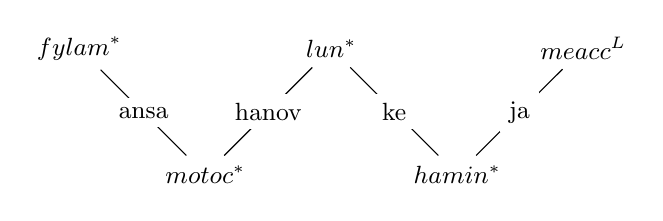
\begin{tikzpicture}[font=\small]
    \node (red) at (0,1.6) {$\ko{fylam}^{*}$};
    \node (head) at (1.6,0) {$\ko{motoc}^{*}$};
    \node (fish) at (3.2,1.6) {$\ko{lun}^{*}$};
    \node (eat) at (4.8,0) {$\ko{hamin}^{*}$};
    \node (cat) at (6.4,1.6) {$\ko{meacc}^{L}$};
    \draw (red) -- node[fill=white] {\ko{ansa}} (head);
    \draw (head) -- node[fill=white] {\ko{hanov}} (fish);
    \draw (fish) -- node[fill=white] {\ko{ke}} (eat);
    \draw (eat) -- node[fill=white] {\ko{ja}} (cat);
\end{tikzpicture}}
\par (a)
\end{minipage}\hfill
\begin{minipage}[c]{0.48\linewidth}
\centering
\resizebox{\linewidth}{!}{%
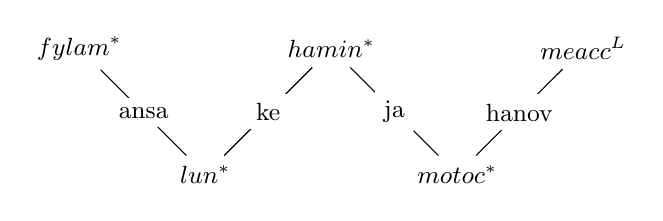
\begin{tikzpicture}[font=\small]
    \node (red) at (0,1.6) {$\ko{fylam}^{*}$};
    \node (fish) at (1.6,0) {$\ko{lun}^{*}$};
    \node (eat) at (3.2,1.6) {$\ko{hamin}^{*}$};
    \node (head) at (4.8,0) {$\ko{motoc}^{*}$};
    \node (cat) at (6.4,1.6) {$\ko{meacc}^{L}$};
    \draw (red) -- node[fill=white] {\ko{ansa}} (fish);
    \draw (fish) -- node[fill=white] {\ko{ke}} (eat);
    \draw (eat) -- node[fill=white] {\ko{ja}} (head);
    \draw (head) -- node[fill=white] {\ko{hanov}} (cat);
\end{tikzpicture}}
\par (b)
\end{minipage}

\medskip
\begin{minipage}[c]{0.48\linewidth}
\centering
\resizebox{\linewidth}{!}{%
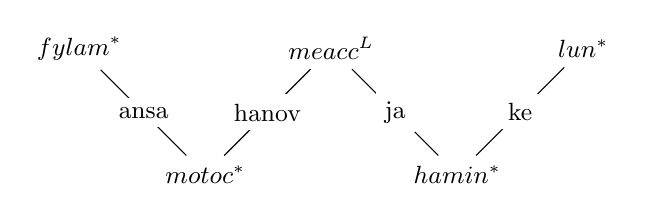
\begin{tikzpicture}[font=\small]
    \node (red) at (0,1.6) {$\ko{fylam}^{*}$};
    \node (head) at (1.6,0) {$\ko{motoc}^{*}$};
    \node (cat) at (3.2,1.6) {$\ko{meacc}^{L}$};
    \node (eat) at (4.8,0) {$\ko{hamin}^{*}$};
    \node (fish) at (6.4,1.6) {$\ko{lun}^{*}$};
    \draw (red) -- node[fill=white] {\ko{ansa}} (head);
    \draw (head) -- node[fill=white] {\ko{hanov}} (cat);
    \draw (cat) -- node[fill=white] {\ko{ja}} (eat);
    \draw (eat) -- node[fill=white] {\ko{ke}} (fish);
\end{tikzpicture}}
\par (c)
\end{minipage}\hfill
\begin{minipage}[c]{0.48\linewidth}
\centering
\resizebox{\linewidth}{!}{%
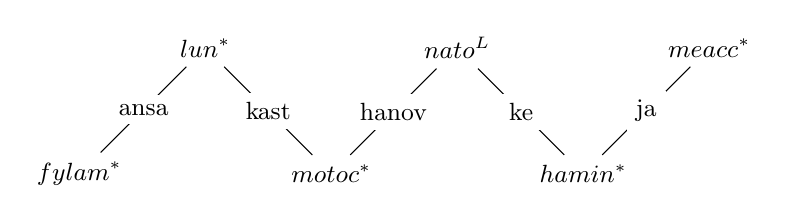
\begin{tikzpicture}[font=\small]
    \node (red) at (0,0) {$\ko{fylam}^{*}$};
    \node (fish) at (1.6,1.6) {$\ko{lun}^{*}$};
    \node (head) at (3.2,0) {$\ko{motoc}^{*}$};
    \node (thing) at (4.8,1.6) {$\ko{nato}^{L}$};
    \node (eat) at (6.4,0) {$\ko{hamin}^{*}$};
    \node (cat) at (8,1.6) {$\ko{meacc}^{*}$};
    \draw (red) -- node[fill=white] {\ko{ansa}} (fish);
    \draw (fish) -- node[fill=white] {\ko{kast}} (head);
    \draw (head) -- node[fill=white] {\ko{hanov}} (thing);
    \draw (thing) -- node[fill=white] {\ko{ke}} (eat);
    \draw (eat) -- node[fill=white] {\ko{ja}} (cat);
\end{tikzpicture}}
\par (d)
\end{minipage}

\medskip
\begin{minipage}[c]{0.48\linewidth}
\centering
\resizebox{\linewidth}{!}{%
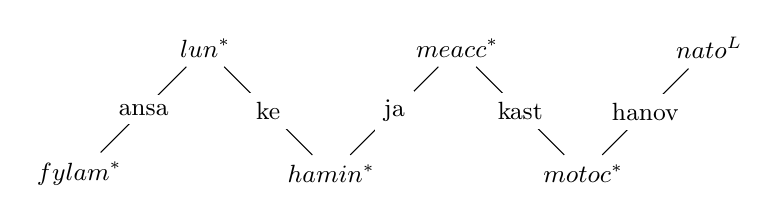
\begin{tikzpicture}[font=\small]
    \node (red) at (0,0) {$\ko{fylam}^{*}$};
    \node (fish) at (1.6,1.6) {$\ko{lun}^{*}$};
    \node (eat) at (3.2,0) {$\ko{hamin}^{*}$};
    \node (cat) at (4.8,1.6) {$\ko{meacc}^{*}$};
    \node (head) at (6.4,0) {$\ko{motoc}^{*}$};
    \node (thing) at (8,1.6) {$\ko{nato}^{L}$};
    \draw (red) -- node[fill=white] {\ko{ansa}} (fish);
    \draw (fish) -- node[fill=white] {\ko{ke}} (eat);
    \draw (eat) -- node[fill=white] {\ko{ja}} (cat);
    \draw (cat) -- node[fill=white] {\ko{kast}} (head);
    \draw (head) -- node[fill=white] {\ko{hanov}} (thing);
\end{tikzpicture}}
\par (e)
\end{minipage}\hfill
\begin{minipage}[c]{0.48\linewidth}
\centering
\resizebox{\linewidth}{!}{%
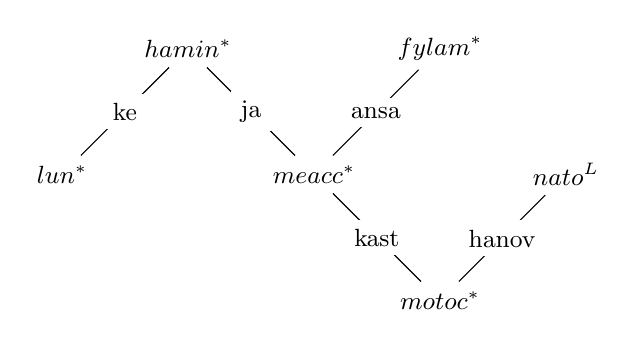
\begin{tikzpicture}[font=\small]
    \node (fish) at (0,1.6) {$\ko{lun}^{*}$};
    \node (eat) at (1.6,3.2) {$\ko{hamin}^{*}$};
    \node (cat) at (3.2,1.6) {$\ko{meacc}^{*}$};
    \node (red) at (4.8,3.2) {$\ko{fylam}^{*}$};
    \node (head) at (4.8,0) {$\ko{motoc}^{*}$};
    \node (thing) at (6.4,1.6) {$\ko{nato}^{L}$};
    \draw (fish) -- node[fill=white] {\ko{ke}} (eat);
    \draw (eat) -- node[fill=white] {\ko{ja}} (cat);
    \draw (cat) -- node[fill=white] {\ko{ansa}} (red);
    \draw (cat) -- node[fill=white] {\ko{kast}} (head);
    \draw (head) -- node[fill=white] {\ko{hanov}} (thing);
\end{tikzpicture}}
\par (f)
\end{minipage}
\caption{「頭が赤い魚を食べる猫」の6解釈}
\label{fig:sakana-six-graphs}
\end{figure}

(a)--(e)は1本の道である．(f)は\ko{meacc}の頂点で分岐し，奇数次数の頂点が4個あるので，一筆書きできない．
例えば\ko{lun}から\ko{nato}までの道と，\ko{fylam}から\ko{meacc}までの辺に分ければ，2つの断片として読み上げられる．

図(a)に冠詞枠と辺の向きを書き加えると，次のようになる．

\begin{center}
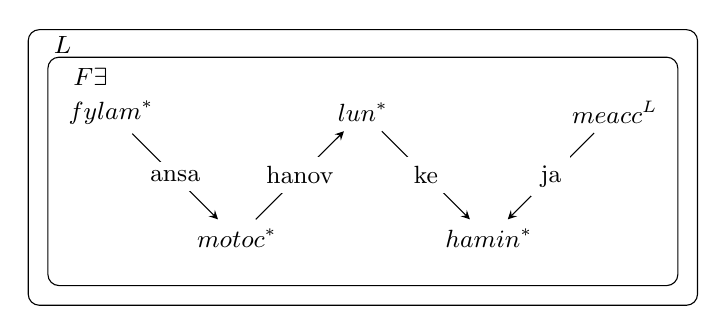
\begin{tikzpicture}[font=\small,>=stealth]
    \draw[rounded corners] (-1.05,-0.85) rectangle (7.45,2.65);
    \draw[rounded corners] (-0.8,-0.6) rectangle (7.2,2.3);
    \node[anchor=west] at (-0.85,2.45) {$L$};
    \node[anchor=west] at (-0.6,2.05) {$F\exists$};
    \node (red) at (0,1.6) {$\ko{fylam}^{*}$};
    \node (head) at (1.6,0) {$\ko{motoc}^{*}$};
    \node (fish) at (3.2,1.6) {$\ko{lun}^{*}$};
    \node (eat) at (4.8,0) {$\ko{hamin}^{*}$};
    \node (cat) at (6.4,1.6) {$\ko{meacc}^{L}$};
    \draw[->] (red) -- node[fill=white] {\ko{ansa}} (head);
    \draw[->] (head) -- node[fill=white] {\ko{hanov}} (fish);
    \draw[->] (fish) -- node[fill=white] {\ko{ke}} (eat);
    \draw[->] (cat) -- node[fill=white] {\ko{ja}} (eat);
\end{tikzpicture}
\end{center}

$F\exists$枠は補助頂点の自由な$F$接辞を存在束縛し，外側の$L$枠は猫の頂点を束縛する．これにより，頭が赤い魚を食べる猫のクラスを作る．$*$は上の図と同じく$F$接辞を表す．\ko{hanov}の両項には材料量への変換$U$を補う．
左から道をたどると，最後の\ko{ja}だけ矢印と逆向きになる．その転置を\ko{meja}で表せば，枠内の線形表示は
\[
    \{\{\ko{fylam ansa motoc hanov lun ke hamin meja }\ko{meacc}^{L}\;F\exists\}\;L\}
\]
となる．

\section{線形文モジュール}
\begin{leftwavybox}
\textbf{完成度（5段階，5が最高）}：誤りの少なさ 3，文章の簡潔さ 3，話題の網羅性 2．
有限の候補生成とソート検査は定まっているが，一般の線形化の規則は未完成である．
\end{leftwavybox}
体系Pでは，以下の2種類の文が(App)規則と(Stl)規則のもとで区別されていた：
\begin{itemize}
    \item 交互型：$t_1\; r_1\; t_2\; r_2\; \cdots\; r_{n-1}\; t_n$（$t$と$r$が交互に並ぶ）
    \item 多引数型：$t_1\; r\; t_2\; t_3\; \cdots\; t_n$（関係$r$の後に引数が並ぶ）
\end{itemize}
線形文モジュールでは，これらを統合して(広義の)線形文を導入し，さらに項の省略（ゼロ照応）を許す．本モジュールの1次的な構文表示はグラフであり（\S\ref{par:flat-kg}），線形文はその1次元への射影である．以下，モジュール全体で使う統語ソートを先に定義し，グラフ表示，線形文のパターン，曖昧性を一括して解消する善意的解釈，グラフと線形文を往復する線形化の順に与える．線形文のパターンは，文字$\{t, R_n,\_\}$（型とは異なる）上のトークン列であり，各記号の意味は以下の通りである：
\begin{itemize}
    \item $t$：個体としての位置
    \item $R_n$：$n$項述語としての位置．$n$はarityを表す添字であり，$n=2$の場合は$n$を省略する．
    \item $\_$（ブランク）：省略された$t$位置（先行詞へのゼロ照応）
\end{itemize}
さらに，$V$型の語がどちらとして解釈されるかを明示するために，任意でトークンに接尾辞$\mathbf{I}$（個体として解釈：$t$位置）または$\mathbf{R}$（関係として解釈：$R$位置）をつけることができる（多くの場合は統語ソートの検査だけで解釈が定まる）．

\paragraph{交互型線形文の由来}
交互型$tRtRt\cdots Rt$は多項関係を1原子として書いたものではなく，関係原子の連言において隣接する原子の共有項を重ねた表記である．例えば$a<b\land b\leq c$を$a<b\leq c$と書くのと同じく，$t_1R_1t_2R_2t_3$は$t_1R_1t_2\mathbin{,}\_R_2t_3$を滑らかに繋いだ形である．この「一筆書き」の形を，線形文モジュールは$t(Rt)^n$として明示的に整形式な構文へ取り込んでいる．背後の1次的なグラフ表示は\S\ref{sec:graph-notation}で，カンマを含む一般の線形化は線形化の節で定義する．


\subsection{統語ソート}
\begin{definition}[統語ソート]
    項$t$の\textbf{統語ソート}$\mathrm{sort}(t) \in A$を，構文から帰納的に定める（意味的な評価は行わない）．
    \begin{enumerate}[label=(\arabic*)]
        \item 定数$a \in F_0$：$\mathrm{sort}(a) = \dom_1 a$（値域ソート）．
        \item 概念$a \in R_1$の項位置での使用：$\mathrm{sort}(a) = a$．
        \item 関数適用$f(t_1,\ldots,t_n)$：$\mathrm{sort} = \dom_{n+1} f$（値域ソート）．引数のソートは検査対象になるが，値には影響しない．
        % \item 名詞化$\cap\{\phi\; L_1\}$：第1スコープの主要部概念．例えば$\cap\{[B^{L_1}], P\text{関連の条件}\; L_1\}$なら$B$．内包条件$P$は参照しない．
        \item 冠詞の結果や部分演算の結果：辞書に結果ソートが指定されていればそれを使い，なければ$\top$とする．
        \item 上記で決まらない項（未知語など）：$\mathrm{sort}(t) = \top$（alkono）．
    \end{enumerate}
\end{definition}
\begin{remark}
    統語ソートは意味的なソートの\emph{上界近似}である：検査を通れば意味的にも整合する（健全）が，内包条件による絞り込みは見ない（不完全）．例えば「偶数の素数」のソートは主要部「素数」から計算され，外延が単元集合であることは使わない．これは静的型付けと同じ設計であり，代わりに，第1スコープの条件$P$が計算不能であっても検査は常に停止する．自然言語の選択制限が外延ではなく主要部で働くこととも整合する．
\end{remark}

\subsection{線形文とパターン}
基本パターンの集合を
\[
    \mathcal B=\{R_0\}\cup\{t(Rt)^k\mid k\geq0\}\cup\{tR_kt^{k-1}\mid k\geq1\}
\]
とする．$\mathcal P$は，$\mathcal B$の各$t$位置を任意にブランク$\_$へ置き換えて得るパターンの集合である．
入力$e=e_1\cdots e_n$に対して，$\mathcal P(e)$を$\mathrm{match}(e,p)$を満たすパターンの集合とする．候補の関係記号に現れる最大アリティと2の大きい方を$K$とする．交互型の関係位置は高々$n$個，多引数型の項位置は高々$K$個なので，長さ$\max(2n+1,K+1)$以下の基本パターンから$\mathcal P(e)$を有限に生成できる．空入力は文として認めない．

候補は，ブランク数，基本パターンの系列（$R_0$，交互型，多引数型の順），系列内の$k$，ブランク位置を昇順に並べた列の順で辞書式に並べる．同じパターンに複数の生成法があれば最小のキーを採る．$p$の優先度は，この有限列$\mathcal P(e)$の0始まりのindexとする．

$p$のブランクを除いた列を$\hat{p}$とする．例えば，$p = tR\_Rt$なら$\hat{p} = tRRt$である．同じ$\hat p$を持つパターンは表層からは区別できないため，どのパターンで読むかは曖昧性の一種である．
\begin{whynot}
「$\mathcal P(e)$内で$p$より前にあり，$\hat q=\hat p$を満たす$q$があれば$p$を除去する」という刈り込みは採らない：同じ入力に対する優先度の高いパターンによる解析が後述の善意的解釈のフィルタで棄却され，より優先度の低いパターンによる解析だけが生き残ることがあるからである．パターンの優先度は，善意的解釈の中のソフト制約（$v_{\mathrm{idx}}$）として働く．
\end{whynot}

(Stl)規則に代わる構文規則は以下の通り：
\[
\infer[\text{(Apl)}]{
    e_1\; e_2\; \cdots\; e_n: \Omega
}{
    n\geq1,\quad\exists p\in\mathcal{P}.\; \mathrm{match}(e_1\cdots e_n, p)
}
\]
ここで$\mathrm{match}$の定義はパターン判定アルゴリズム（次段落）による．参考として，非ブランク列$\hat p$の長さが3以下の場合について，最優先パターンの例を挙げる（他のフィルタがすべて通る場合に選ばれるもの）：
\begin{itemize}
    \item $\text{length} = 1$：$t,\; R_0$
    \item $\text{length} = 2$：$tR_1,\; \_Rt,\; \_R\_R\_$
    \item $\text{length} = 3$：
    \begin{align*}
        & tRt,\; \_R_3tt,\;\_R\_Rt,\; \_RtR\_,\\
        & tR\_R\_,\; \_R\_R\_R\_
    \end{align*}
\end{itemize}

\paragraph{パターン判定アルゴリズム}
線形文$e_1\cdots e_n$の各トークンについて，候補記号の集合$m(e_i)$を次の順に定める．
\begin{enumerate}
    \item 接尾辞$\mathbf I$があれば$m(e_i)=\{t\}$．接尾辞$\mathbf R$があれば，辞書でアリティ$k$が定まる述語では$\{R_k\}$，未知語では$\{R_2\}$とする．
    \item 接尾辞がなく辞書にある場合，$R_0$は$\{R_0\}$，$R_1$は$\{t,R_1\}$，$F_0$は$\{t\}$，$R_k$（$k\geq2$）は$\{R_k\}$とする．正のアリティの関数語は，引数を与えて項を作るまで単独の候補を持たない．
    \item 型が定まった複合項は$\{t\}$とする．未知語は$\{t,R_2\}$とする．
\end{enumerate}
候補集合に対する連結を$A\circ B=\{uv\mid u\in A,\ v\in B\}$と定める．このとき
\[
    \mathrm{match}(e_1\cdots e_n,p)\iff
    \hat p\in m(e_1)\circ\cdots\circ m(e_n).
\]

\subsection{善意的解釈}
線形文モジュールの線形文には，(1) パターンの選択，(2) 関係の転置（$r$を$r^\trans$として読む），(3) ブランクの先行詞選択，という3種類の曖昧性がある．口語で読むときの心理的な動きを再現するように，これらを一括して解消する手続きを\textbf{善意的解釈}と呼ぶ．
\begin{whynot}
素朴には「文を真にする解釈を選ぶ」（真にする割り当ての集合が包含順序で極大な読みを選ぶ）ことが考えられるが，採らない．もっともらしさだけを最大化すると読みは恒真に向かって弱くなり，文が情報を運ばなくなるからである．逆に「矛盾しない限り最強の読みを選ぶ」という方針は，相互構文の解釈について提案されたStrongest Meaning Hypothesis \cite{smh}と同型だが，これも単独では否定環境での強弱の反転などの問題を持つ．そこで善意は真理にではなく\emph{整形式性}に向ける：まず統語的に検査できるハードフィルタで候補を絞り，残った候補を違反ベクトルの辞書式順序で比較する．
\end{whynot}

\begin{definition}[先行詞リストと走査]
    \textbf{先行詞リスト}$\Delta$は指示子とソートプロファイルの対を言及の新しい順に並べる．初期値は談話モジュールから受け取る．線形文の項位置を左から読み，項・ブランク・指示詞の参照先を先頭へ移す（未登場なら挿入する）．関係語だけでは更新しない．位置$i$を読む直前のリストを$\Delta_i$とする．同じ$F$ラベルの項には同じ仮指示子を使い，新しい$F$同値類には新しい仮指示子を割り当てる．これらは陳述更新の証人規則で使う指示子と共通にする．
\end{definition}

\begin{definition}[解析]
    線形文$e_1\cdots e_n$と先行詞リスト$\Delta$に対して，\textbf{解析}とは組$\alpha = \langle p, \tau, g\rangle$である．
    \begin{itemize}
        \item $p \in \mathcal P$：$\mathrm{match}(e_1\cdots e_n, p)$を満たすパターン．
        \item $\tau$：$p$の各$R$位置に対する転置フラグ（$0$なら$r$，$1$なら$r^\trans$として読む）．
        \item $g$：$p$の各ブランクへの先行詞の割り当て（対応する$\Delta_i$の要素を値に取る）．
    \end{itemize}
    解析$\alpha$の\textbf{読み}$\lbb\alpha\rbb$は，$p$の型（交互型・多引数型）に従って構成される連言である．
\end{definition}

\begin{definition}[ハードフィルタ]
    解析$\alpha$は以下をすべて満たすときに限り候補となる．
    \begin{enumerate}[label=(H\arabic*)]
        \item \textbf{ソート整合}：読みに現れる各$n$項原子$r(t_1,\ldots,t_n)$について，転置を反映した引数順で
        \[
            \mathrm{sort}(t_i)\preceq\dom_i r^\tau\qquad(i=1,\ldots,n)
        \]
        を要求する．$n=0$では検査する引数はない．有限の辞書データ上で$\preceq$を到達可能性として検査する．自由転置は2項原子で両項を交換する操作とし，それ以外のアリティでは$\tau=0$のみを用いる．
        \item \textbf{共項排除}：ブランクである引数$t_i$は，同じ原子の他のどの引数$t_j$（$j\ne i$）とも同じ指示子に解決しない．1項原子ではこの制約は空虚である．
    \end{enumerate}
\end{definition}
\begin{remark}
    共項排除は自然言語の束縛条件B（``John$_i$ hit him$_i$''の禁止）に対応する統語的制約である．ブランクにのみ課されることに注意：再帰的な読みが欲しければ$A^{F_1}RA^{F_1}$と同じラベルを明示すればよく，再帰代名詞に相当する装置は不要である．両引数がブランクの場合は，両者が同一の先行詞に解決されないことを意味する．
\end{remark}
% 2026-09-05裁定：ソート整合の「共通下位概念の存在」への緩和は採らない（分類文は指示詞で先行詞を明示する．実践編「文型と線形文」）．

\begin{definition}[ランキング]
    ハードフィルタを通った解析$\alpha$に対して，違反ベクトル
    \[
        v(\alpha) = \langle v_{\mathrm{red}}(\alpha),\; v_{\tau}(\alpha),\; v_{\mathrm{rec}}(\alpha),\; v_{\mathrm{idx}}(\alpha),\; v_{\mathrm{pos}}(\alpha)\rangle
    \]
    を以下で定める．\textbf{善意的解釈}とは，$v$を\emph{辞書式順序}（左の成分ほど優先）で最小化する解析（の集合）である．
    \begin{enumerate}[label=(\arabic*)]
        \item \textbf{非冗長性}$v_{\mathrm{red}}$：転置を反映した読みの連言肢を$C_1,\ldots,C_m$とし，
        \[
            v_{\mathrm{red}}=m-\min\Bigl\{|J|\;\Big|\; J\subseteq\{1,\ldots,m\},\;
            \bigwedge_{j\in J}C_j\vdash_{\mathrm{sort}}\bigwedge_{j=1}^{m}C_j\Bigr\}
        \]
        とする．$\vdash_{\mathrm{sort}}$は同一原子とソート・$\preceq$由来の含意だけを使う．元の情報を保って削除できる連言肢の最大数を罰する．
        \item \textbf{自由転置数}$v_{\tau}$：ソートが強制しない転置の個数．すなわち，両方の語順がソート整合であるにもかかわらず$\tau_j = 1$を選んだ$R$位置の個数．ソートが転置を強制する場合（$\tau_j = 0$がH1に反する場合）は数えない．
        \item \textbf{新近性}$v_{\mathrm{rec}}$：各ブランク$i$について，$g$の値の$\Delta_i$上での位置（先頭を$0$とする）を左から並べた列．列同士は辞書式に比較する（先に読むブランクほど優先して新しい先行詞を取る）．
        \item \textbf{パターン優先度}$v_{\mathrm{idx}}$：$p$の入力ごとの有限列$\mathcal{P}(e)$におけるindex．
        \item \textbf{転置の配置優先度}$v_{\mathrm{pos}}$：$\tau$の辞書式順序．
    \end{enumerate}
    成分の順序は，読み手が話者に帰属させる非合理性の重大さの降順である：発話の一部を空虚にする読み（1）は，無標語順からの無動機な逸脱（2）より重く，それは顕著でない先行詞の選択（3）より重く，それは頻度の低いパターンの使用（4）より重い．(5)は(1)--(4)までで複数選択肢が残るときのタイブレークに使う．
\end{definition}
\begin{remark}[連言肢ごとの冗長性]
    各連言肢が他の連言肢から従うかを独立に数える方式もある．この方式では同じ原子を2回書くと両方が該当し，罰点は2になる．上の削除数による定義では1個を残すため，罰点は1である．
\end{remark}
\iffalse
\begin{remark}[強さのタイブレーク]
    上のランキングで同順位が残った場合に限り，辞書の公理のもとでの含意$\lbb\alpha\rbb \vdash \lbb\alpha'\rbb$による半順序で\emph{極小}（最強）の読みを選好する（SMH）．ただしこの順序で比較可能になるケースは少なく，実質的な仕事の大半は(1)--(4)で終わる．含意判定は$\preceq$由来の含意に制限すれば決定可能である．
\end{remark}
% (1)-(4)だけだと転置の"配置"は特定できないのでSMHにfall backする．aRbRcを考えてみると良い．
\fi

\begin{proposition}[計算可能性]
    有限の辞書データと先行詞リストを用い，対象のアリティに対するソート検査・H1・H2が定まっているとする．入力ごとの$\mathcal P(e)$，転置の選択，先行詞の選択はいずれも有限であり，冗長性は有限個の連言肢の部分集合を調べて計算できる．これらの検査が計算可能なら，善意的解釈も計算可能である．候補が空のとき，その線形文は非文である（誤りが検出できることは，すべてを救済する真理ベースの善意に対する利点である）．最小元が複数あるとき，その文は多義である．
\end{proposition}
\begin{remark}[貪欲アルゴリズムとの関係]
    定義は解析全体にわたる大域的な最小化だが，左から読み進めながら各ブランクを「フィルタを通り，冗長を生まない，最も新しい先行詞」に解決する貪欲アルゴリズムは，多くの場合に同じ結果を与える．両者がずれる例として，先の選択が後で冗長性を強制する文がある（後述の$R^n$の例）．そのとき定義は大域的な整合性（$v_{\mathrm{red}}$の優先）を取る．読解の心理としては，貪欲に読んで行き詰まったら読み直す，という袋小路文（garden path）の再現になっている．
\end{remark}

\begin{example}[ラベルを共有する相互文]
    $R$は両方向のソート検査を通り，非対称な語彙関係を追加で仮定しないものとする．線形文$A^{F_1}RA^{F_2}RA^{F_1}$を考える．
    \begin{itemize}
        \item 転置なし：$A^{F_1}RA^{F_2}\land A^{F_2}RA^{F_1}$．冗長性は0，自由転置数は0．
        \item 後半を転置：$A^{F_1}RA^{F_2}\land A^{F_1}RA^{F_2}$．冗長性は1，自由転置数は1．
    \end{itemize}
    ランキングは転置なしの相互的な読みを選ぶ．
\end{example}

\begin{example}
    別の先行詞$\delta_2$だけがある状態で$A^{F_1}RR$を読み，$F_1$に対応する指示子を$\delta_1$とする．パターンは$tR\_R\_$である．最初のブランクを読む直前の順序は$[\delta_1,\delta_2]$だが，H2により$\delta_1$を取れないため$\delta_2$を選ぶ．次は$[\delta_2,\delta_1]$のもとで$\delta_1$を選ぶ．両対象が$R$のソートを満たせば，読みは$\delta_1$から$\delta_2$，$\delta_2$から$\delta_1$への2原子になる．
\end{example}

\begin{example}\label{ex:rn}
    $R^n$を，先行詞の順序が$[\delta_1,\delta_2,\delta_3,\delta_4]$のもとで読む．以下ではすべての先行詞が$R$の両項のソートを満たし，異なる原子間にソート由来の含意がない場合を考える：
    $R$のみを$n$回並べた線形文はパターン$(\_R)^n\_$にマッチし，読みの骨格は隣接する$n+1$個のブランクを結ぶ原子列である．ハードフィルタは「隣接ブランクの指示対象が異なる」ことだけを要求するので，冗長ゼロの読みは「頂点集合$\{\delta_1,\delta_2,\delta_3,\delta_4\}$上の完全有向グラフにおける，辺を繰り返さない歩道」と1対1に対応する．したがって$|\Delta| = k$のとき冗長ゼロが可能なのは$n \leq k(k-1)$（$k=4$で$12$）原子までであり，それを超えると$v_{\mathrm{red}} > 0$が強制される．$n = 12$では善意的解釈は
    \[
        \delta_1\,R\,\delta_2\,R\,\delta_1\,R\,\delta_3\,R\,\delta_1\,R\,\delta_4\,R\,\delta_3\,R\,\delta_4\,R\,\delta_2\,R\,\delta_3\,R\,\delta_2\,R\,\delta_4\,R\,\delta_1
    \]
    という解決済み指示子のオイラー路を与える（新近性を優先しつつ，行き詰まらない範囲で最新の先行詞を選ぶ）．純粋な貪欲（大域的な実行可能性を見ない）は第7ブランクで$\delta_1$を選び，第7原子で重複$\langle \delta_1, \delta_4\rangle$が強制される．定義は$v_{\mathrm{red}}$を$v_{\mathrm{rec}}$より優先するので，第7ブランクで新近性を犠牲にして$\delta_3$を選ぶ方が採られる．
\end{example}

\begin{remark}[往復条件]
    善意的解釈は省略形から完全な読みへの写像である．逆方向として，読み$m$から最優先パターン・最小トークン数の線形文を生成する\textbf{標準形}関数$\mathrm{nf}(m)$を（生成規則の側で）定義し，往復条件
    \[
        \lbb \mathrm{nf}(m) \rbb = m
    \]
    を体系の設計要件とする．$\mathrm{nf}$は現時点では未定義であり，生成規則を与えるまでは往復条件を定理として用いない．同じ内容に対する複数の表層形（例えば$tRR$と$RtR$のパターン）のどちらが標準かは$\mathrm{nf}$が定め，解釈側のランキングと生成側の規則はこの条件を満たすように共設計される．条件の検証は，内容をランダム生成して$\mathrm{nf}$と善意的解釈を往復させるproperty-basedテストとして機械化できる．なお意味論そのものは省略なしの完全形（体系P）にのみ与えられており，善意的解釈は「省略形$\to$完全形」の前処理層に閉じている．前処理層の複雑さは意味論には漏れない．
\end{remark}

\begin{remark}[非単調性と保存規約]
    マッチング候補$m(e_i)$はトークンの辞書登載の有無に依存するため，辞書が成長すると過去のテキストの善意的解釈が変わりうる（未知語として$[t, R]$だったものが登載により固定され，勝つパターンが変わる）．長期運用のため，保存を目的とするテキストでは接尾辞$\mathbf{I}/\mathbf{R}$を必須とするか，テキストに辞書のバージョンを紐付けることを規約とする．
\end{remark}
% \cite{smh} Dalrymple et al. 1998, Reciprocal expressions and the concept of reciprocity.
% \cite{blutner} Blutner 2000, Some aspects of optimality in natural language interpretation.
\iffalse
\subsection{パターンマッチングの例}
\noindent
以降，$a_i\in A$，$b_i\in B$，$A \cap B = \emptyset$，$R_i \subseteq A \times B$，$S_i \subseteq A \times A$とする．$(\bullet)^c$は補集合（関係の否定）を表す．
\begin{remark}
    同じ文中で導入した個体も$\Delta$に追加されるようにすべきではないだろうか．
\end{remark}
\begin{table}[H]
\centering
\begin{tabular}{ccccc}
    \toprule
    先行詞 & 構文 & パターン & 代入後 & 備考\\
    \midrule
    $\Delta = \emptyset$ & $aRb$ & $tRt$ & $aRb$ \\
    $\Delta = \emptyset$ & $bRa$ & $tRt$ & $aR^\trans b$ & ソート整合性\\
    $\Delta = \emptyset$ & $aS$ & $tR\_$ & $aSa$ & \\
    $\Delta = \emptyset$ & $Sa$ & $\times$ & $\times$ & 代入候補なし\\
    $\Delta = [a_1]$ & $Sa_2$ & $\_Rt$ & $a_1Sa_2$ & \\
    $\Delta = [a_1]$ & $a_2S$ & $tR\_$ & $a_2Sa_2$ & 親近性\\
    $\Delta = \emptyset$ & $a_1Sa_2Sa_1$ & $tRtRt$ & $a_1Sa_2 \land a_2Sa_1$ & \\
    $\Delta = [a_1]$ & $a_2SSa_2$ & $tR\_Rt$ & $a_2Sa_1 \land a_1Sa_2$ & $a_2$の代入は冗長\\
    $\Delta = [a_1]$ & $a_2SS^ca_2$ & $tR\_Rt$ & $a_2Sa_1 \land a_1S^ca_2$ & $a_2$の代入は矛盾\\
    $\Delta = [a_1]$ & $a_2SS$ & $tR\_R\_$ & $a_2Sa_2 \land a_2Sa_1$？$a_2Sa_1 \land a_1Sa_2$？ &\\
    \bottomrule
\end{tabular}
\end{table}
\fi
\iffalse
\subsection{線形化と一筆書き}
グラフから線形文への射影を定義する．交互型線形文はグラフ上の歩道の読み上げであり，歩道内部の共有項は項の重なりとして，歩道間の共有項は同じラベルまたはブランク照応として現れる．

\begin{definition}[なぞり語列]
    $G$の無向化上の歩道
    \[
        W=v_0e_1v_1\cdots e_nv_n
    \]
    に対し，\textbf{なぞり語列}$\operatorname{tr}(W)$は，頂点ラベルと辺ラベルを歩道順に交互に並べたものとする．
    辺$e_i$を$s(e_i)$から$t(e_i)$へたどるときは$\ell_E(e_i)$を，逆向きにたどるときは$\mathsf{me}\,\ell_E(e_i)$を置く．
    後者の$\mathsf{me}$は，H1が向きを一意に定める会話形では省略できるが，保存形では明示する．
\end{definition}

\begin{definition}[線形分解]
    $G$の辺集合を，辺を反復しない歩道$W_1,\dots,W_k$の辺集合へ直和分割したものを\textbf{線形分解}という．
    対応する線形表示を
    \[
        \operatorname{lin}_{\mathcal W}(G)
        :=\operatorname{tr}(W_1)\mathbin{,}\cdots\mathbin{,}\operatorname{tr}(W_k)
    \]
    とする．ここでカンマは各断片が表す原子列の連言であり，談話モジュールの意味で複数の文・発話へ分ける標識ではない．線形分解に先立ち各頂点$v$に一意なラベル$i_v$を割り当て，$\operatorname{tr}(W_j)$に現れる同一頂点の全出現へ同じ$F_{i_v}$を付ける（同じ裸語の別出現は別個体になるため）．ブランクを用いる場合は，その解決先が$i_v$の頂点であることも線形分解のデータに含める．
\end{definition}

\begin{proposition}[線形化の保存性]
    $G$がソート整合的で，逆向きにたどる辺が正しく転置されているなら，任意の線形分解$\mathcal W$について
    \[
        \lbb\operatorname{lin}_{\mathcal W}(G)\rbb=\lbb\Phi_G\rbb
    \]
    である．
\end{proposition}
\begin{proof}
    各辺はただ一つの歩道に一度だけ現れるため，線形表示が作る原子の多重集合は$\Phi_G$の連言肢と一致する．共有頂点は，歩道内部では項の重なりとして，異なる歩道間では同じラベルまたはブランク照応として保存される．あとは連言の結合・交換法則による．
\end{proof}

すべての辺を一つの歩道で覆う線形分解を\textbf{一筆線形化}という．一筆線形化が存在してもそれを選ぶ義務はなく，グラフのまま書くことも，説明上分かりやすい複数断片に分けることもできる．ただし，発話・筆記では共有項を反復せず視点を滑らかに移せるため，一筆線形化が推奨される．

\begin{proposition}[一筆書き判定]
    辺を一つ以上持つ連結な関係グラフ$G$が一筆線形化を持つのは，矢印を無視した多重グラフにおいて奇数次数の頂点が$0$個または$2$個のとき，かつそのときに限る．
\end{proposition}

非連結な図は連結成分ごとに少なくとも一断片を要する．一つの連結成分に奇数次数頂点が$o$個あるとき，全辺を反復なしに覆うために必要な歩道の最小数は$\max(1,o/2)$である．
したがって一筆書きできないグラフも常に複数断片へ線形化でき，断片をカンマで繋げばよい．辺を重ねて無理に一筆書きにすると同一原子の反復を生じ，$v_{\mathrm{red}}$により非標準となる．
\fi

\section{指示詞モジュール}\label{subsec:demonstrative}
\begin{leftwavybox}
\textbf{完成度（5段階，5が最高）}：誤りの少なさ 3，文章の簡潔さ 4，話題の網羅性 3．
順位による参照と主要部による制限は定まっているが，前方照応の処理が未確定である．
\end{leftwavybox}
基本体系では，$A^{F_1}\;R\;A^{F_1}$のように同じラベルを付けて同じ項を指定できる．指示詞は，参照時点の先行詞リスト$\Delta$の「$n$個前」を指定する．本節では言及の新しい順を用い，先頭を1個前と数える．

\begin{definition}[指示詞トークン]
    指示詞$\dem{n}{B}$は正整数$n$と主要部概念$B\in R_1$からなる．主要部を省く場合は$\dem{n}{-}$と書く．位置$i$のトークンを読む直前のリストを
    $\Delta_i=[(\delta_1,\Gamma_1),\ldots,(\delta_k,\Gamma_k)]$とする．
    \begin{itemize}
        \item パターンは$m(\dem{n}{B})=\{t\}$．
        \item $1\leq n\leq k$なら参照先を$\delta_n$に解決する．可能性$(w,g)$における値は，主要部があれば
        \[
            \mathrm{the}\bigl(\{g(\delta_n)\}\cap\lbb B\rbb_c^{w,g}\bigr)
        \]
        とし，主要部がなければ$g(\delta_n)$とする．番号が範囲外，割り当てが未定義，または交差が空なら未定義となり，それを含む原子文は偽となる．
        \item 統語ソートは$B$．主要部がなければ$\Gamma_n$を用い，H1はそのいずれかのソートが要求ソート以下なら通る．主要部によってリストを絞ってから数える操作はしない．
        \item 解決後に$(\delta_n,\Gamma_n)$を先頭へ移す．同じ指示子を重複して挿入しない．解決した参照先と主要部はそのトークンに保持し，後の並べ替えで選び直さない．
    \end{itemize}
\end{definition}
\begin{example}
    $\Delta_i=[(\delta_3,\Gamma_3),(\delta_1,\Gamma_1),(\delta_2,\Gamma_2)]$なら，$\dem{2}{-}$は$\delta_1$を取り，リストは$[(\delta_1,\Gamma_1),(\delta_3,\Gamma_3),(\delta_2,\Gamma_2)]$になる．続く$\dem{2}{-}$は$\delta_3$を取る．同じ番号でも参照時点の順序によって対象が変わる．
    $g(\delta_1)$が小麦で，食べ物の外延に属し，数の外延に属さないとする．この小麦を「その食べ物」と呼べば値は小麦であり，「その数」と呼べば未定義となる．
\end{example}
\begin{remark}
    指示詞はブランクでないため，共項排除H2と新近性の違反値$v_{\mathrm{rec}}$の対象にならない．直前に言及した対象への再帰的な参照は$\dem{1}{-}$で指定できる．同じ対象を別の主要部で指すと，その主要部のソートでH1を検査する．
    別の規則で整理した指示子列を使う場合にも，列を定めてからその$n$番目を取る．その列の構成・更新規則は個別に定める．
\end{remark}
\begin{proposition}
    有限の先行詞リストと計算可能なソート検査が与えられれば，指示詞の解決は計算可能である．
\end{proposition}
\begin{proof}
    各解析で参照時点のリストの$n$番目を取り，先頭へ移す有限操作であり，指示詞自身は先行詞選択の分岐を増やさない．
\end{proof}

\paragraph{前方指示（\ko{lon}系列）}
5-2の\ko{lon}/\ko{lota}系列は，後続の導入を予告する前方照応である．まだ導入されていない指示先を直ちに評価すると原子文が偽になるため，通常の\ko{sen}系列と同じ即時評価には載せられない．

現行方針は，談話モジュール側に未確定の指示を保持し，後続の導入で一意化する方式である（2026-09-07暫定）．2パスで文全体を再解釈する案は採らない．ただし，この方針だけでは増分走査への接続は完成しない．
% @issue KONO-0032
\todo{未確定指示子の導入・評価保留・確定規則を談話モジュールに書く．保留した指示と後続導入の対応，ソート制約の保持，確定時の保留原子の評価，未解決のまま談話を閉じた場合を定める．未定義項を含む原子文を偽にする既存規約との適用範囲も分ける．}

\section{談話モジュール}\label{subsec:systemD}
\begin{leftwavybox}
\textbf{完成度（5段階，5が最高）}：誤りの少なさ 2，文章の簡潔さ 4，話題の網羅性 3．
状態更新と疑問のスコープは定まっているが，前方照応と動的接続詞の処理が未確定である．
\end{leftwavybox}
文種，発話状況，情報状態の更新を扱う．以下の談話区間と解答先の指定は暫定とする．

\begin{definition}[辞書の拡張]
    辞書に，文種の集合$M_{\mathrm{utt}}$，慣用表現の集合$N$，談話指示子の集合$X_\delta\subseteq X$，指標詞定数の集合$J\subseteq F_0$を加える．$J$には「私」「今」「ここ」などが属する．
\end{definition}
\begin{definition}[発話]
    発話を次の規則で帰納的に定める．
    \[
    \infer[\text{(Utt-S)}]{\langle\mathsf S,\phi\rangle:\mathrm{Utt}}{\phi:\Omega}
    \qquad
    \infer[\text{(Utt-Q)}]{\langle\mathsf Q,\phi,I\rangle:\mathrm{Utt}}
          {\phi=\{\theta\;E_I\}\quad\text{または}\quad(\phi:\Omega,\ I=\emptyset)}
    \]
    \[
    \infer[\text{(Utt-A)}]{\langle\mathsf A,r;j\rangle:\mathrm{Utt}}{r\in\mathrm{Ans},\quad j\in\mathbb N\cup\{\_\}}
    \qquad
    \infer[\text{(Utt-N)}]{\langle\mathsf N,n\rangle:\mathrm{Utt}}{n\in N}
    \]
    \[
    \infer[\text{(Utt-D)}]{\langle\mathsf D,u_1,\ldots,u_n\rangle:\mathrm{Utt}}
          {u_i:\mathrm{Utt}\quad(i=1,\ldots,n)}
    \]
    $E$を持つ疑問では$I$はその束縛ラベル列であり，$E$を持たない$\Omega$型の式は極性疑問として扱う．$j$は解答先の疑問発話IDである．$j=\_$は省略できる．解答$\mathrm{Ans}$には式$\psi:\Omega$，有限な項指定$a:\Lambda\rightharpoonup\mathrm{Rep}(V)$，極性応答$+,-$を含める．談話は発話の有限列であり，$\mathsf D$はその局所区間を作る．
\end{definition}

\begin{definition}[文脈]
    文脈は$c=\langle\kappa,\rho,D_\delta,s,\Theta,\Delta,H\rangle$である．
    \begin{itemize}
        \item $\kappa$：話者・聞き手・時刻・場所などの発話状況．指標詞への割り当て$\rho_\kappa\in\mathrm{Fin}(J,\mathcal M)$を定める．
        \item $\rho$：語彙割り当て．
        \item $D_\delta\subseteq X_\delta$：有限な指示子定義域．空の情報状態でも保持する．
        \item $s\subseteq W\times\mathcal M^{D_\delta}$：情報状態．可能性$\langle w,g\rangle$は世界と談話指示子への値割り当ての対である．
        \item $\Theta$：問いレコード$\langle j,I,Q\rangle$のスタック．$j$は発話ID，$I$は項ラベル列，$Q\subseteq\wp(s)$は包含について下方閉な問いの内容である．
        \item $\Delta\in\mathrm{List}(X_\delta\times\mathrm{SortProfile})$：指示子と既知ソートの対を言及の新しい順に並べた先行詞リスト．同じ指示子は高々1度だけ現れる．
        \item $H$：発話履歴．各記録は一意なID，発話状況，構文，指示詞・ブランクの解決済み参照先，応答先，所属する談話区間を持つ．
    \end{itemize}
    $\Delta$に現れる指示子はすべて$D_\delta$に属する．文脈の全体を$C$とする．
\end{definition}

\begin{definition}[内容と更新]
    内容式の評価を$\lbb\phi\rbb_c^{w,g}:=\lbb\phi\rbb_{\rho\vll\rho_w\vll\rho_\kappa,\;\sigma\vll g}$，発話による更新を$\lbb u\rbb:C\rightharpoonup C$と書く．内容式の真理値は可能性ごとに定まり，更新はその情報を文脈へ反映する．各基本発話の処理時には新しいIDで$H$に記録する．問いの指示詞は質問時の走査で解決した指示子を保ち，提示命題にある指標詞は質問時の$\kappa$で固定し，解答として新たに与えられた式や項の指標詞は解答時の$\kappa$で評価する．
\end{definition}

\begin{definition}[指示子の導入と証人]\label{def:discourse-witness}
    以下の$F$導入規則が適用される項位置では，定数$c\in F_0$への初回言及も，単元スコープ$\{\lbb c\rbb_c^{w,g}\}$を持つ$F$項として指示子を導入する．定数の値が未定義ならこのスコープは空とする．同じ発話内の同じ定数トークンは同じ導入を共有する．異なる発話での再導入を許し，値の一致だけで指示子を統合しない．指標詞の値は導入した発話の状況で固定する．この単元スコープは先行詞を立てるためのもので，定数を関数の引数に評価する規則は変えない．
    線形文の善意的解釈で解析を選び，ブランク・指示詞を指示子に解決した内容を$\phi$とする．他の冠詞に束縛されていない最外層の$F$接辞付き項の同値類へ，最初の出現順に新しい指示子$\delta_i$を1度ずつ割り当てる．それらの集合を$B_\phi$とする．$\phi[g']$は，この$F$接辞付き項を$g'(\delta_i)$で置き換えた式である．
    \[
        \mathrm{Wit}_{w,g}(\phi)=
        \{g':B_\phi\to\mathcal M\mid g'\text{は各第1スコープを満たし，}
                         \lbb\phi[g']\rbb_c^{w,g}=1\}.
    \]
    値による置換はメタ言語上の評価操作とする．これらの新規項を各第1スコープ上で存在閉包した内容を$\phi^\exists$と書く．導入がなければ，これは$\phi$が真のとき$\{\emptyset\}$，偽のとき$\emptyset$である．否定や別の冠詞の内部で束縛された項は，この規則では外へ導入しない．
    $\Delta$には第1スコープの主要部ソートを保存する．$F_i$のラベルは内容式内の共有を決め，指示詞の番号は走査時点の$\Delta$上の位置を指定する．既存指示子への言及は，線形文の走査で得た順に先頭へ移す．
\end{definition}
\begin{remark}
    線形解析が決めるのは，どの項出現が同じ指示子を指すかである．$\mathrm{Wit}$はその解析を入力として，各世界で内容を真にする個体の割り当てを求める．
\end{remark}
\memo{選言・条件文の内部から後続へ到達できる指示子の範囲は未確定である．最外層の導入規則を一般の動的接続詞へ拡張する際に定める．}

\begin{definition}[問いの文脈への移し替え]
    更新前後の情報状態を$s,s'$とし，$\pi(\langle w,g'\rangle)$を更新前の$D_\delta$への制限とする．$\pi[s']\subseteq s$である更新では，各問いを
    \[
        Q\!\upharpoonright\!s':=\{v\subseteq s'\mid\pi[v]\in Q\}
    \]
    へ移す．指示子の導入がなければ$Q\cap\wp(s')$となる．問いのID，項ラベルとスタック内の順序は保存する．
\end{definition}

\begin{definition}[発話の更新]
    \leavevmode
    \begin{itemize}
        \item \textbf{陳述}：$\langle\mathsf S,\phi\rangle$は
        \[
            s'=\{\langle w,g\vll g'\rangle\mid\langle w,g\rangle\in s,
                           \ g'\in\mathrm{Wit}_{w,g}(\phi)\}
        \]
        へ更新し，$D_\delta$に新規指示子を加え，指示子を登録して問いを$s'$へ移す．
        \item \textbf{疑問}：$\langle\mathsf Q,\phi,I\rangle$の発話IDを$j$とする．$\phi=\{\theta\;E_I\}$の場合，その第1スコープを可能性ごとに$S_{w,g}\subseteq\mathcal M^I$として求め，
        \[
        \begin{split}
            U_e(S,\psi)&=\{\langle w,g\rangle\in s\mid H(e,w),\quad
                  e\in\rho_{I,\sigma\vll g}(C)(S_{w,g},\psi)\},\\
            E^D_s(S,\psi)&={\downarrow}\{U_e(S,\psi)\mid e\in\Sit\},\\
            Q_{\phi,I,s}&=E^D_s(S,\theta^\exists)
        \end{split}
        \]
        を$\langle j,I,Q_{\phi,I,s}\rangle$として積む．これは冠詞$E$の「正確検証者を世界化して下方閉包を取る」操作を，世界と指示子割り当ての対へ持ち上げたものである．$\theta^\exists$は，問われる$E_i$の項を残し，他の新規$F$項だけを存在閉包した内容を表す．$E_i$の量化範囲は$S_{w,g}$であり，$\mathcal M^I$全体には広げない．
        $E$を持たない$\phi:\Omega$は極性疑問とし，$T=\{\langle w,g\rangle\in s\mid\lbb\phi^\exists\rbb_c^{w,g}=1\}$に対する$Q=\wp(T)\cup\wp(s\setminus T)$を積む（$E_{\mathrm{pol}}$）．
        情報状態と$D_\delta$は変えない．既存指示子への言及順は$\Delta$へ反映するが，新規の仮指示子は登録しない．履歴には解決済みの提示構文，束縛ラベル，第1スコープの構文と発話状況を保存する．
        \item \textbf{解答}：$\langle\mathsf A,r;j\rangle$は，$j$があればそのIDの問いを，$j=\_$なら$\Theta$の先頭を選ぶ．該当する開いた問いがなければ未定義となる．選んだ$\langle j,I,Q\rangle$について，$E$付きの提示構文ならその本体$\theta$を，極性疑問なら元の$\Omega$型の式を$\phi$とし，解答を次の内容式へ展開する．
        \[
            \psi_r=\begin{cases}
                r & r:\Omega,\\
                \phi(a) & r=a\text{（項指定）},\\
                \phi & r=+,\\
                \lnot\phi & r=-.
            \end{cases}
        \]
        項指定は$\mathrm{dom}(a)\subseteq I$を要する．$\phi(a)$では，指定した各値が質問時の第1スコープを満たすという条件を残し，未指定の位置はその第1スコープ上で存在閉包する．極性応答は極性疑問にのみ用いる．
        束縛スコープを持たない式には$S_{w,g}=\{\emptyset\}$として$E^D_s(\psi):=E^D_s(S,\psi)$と略記する．まず$s_0=s\cap\bigcup E^D_s(\psi_r^\exists)$とする．極性応答では質問時に固定した提示命題の真理集合$T$を現文脈へ移し，肯定は$s_0=s\cap T$，否定は$s_0=s\setminus T$とし，極性応答では新しい指示子を導入せず$s'=s_0$とする．その他の解答では，$s_0$の各可能性について閉包前の$\psi_r$の証人を求め，新規指示子を$D_\delta$へ加えて登録し，$s'$を得る．更新前への射影$\pi[s']$が$Q$に属せば完全解答として選んだレコードだけを除き，そうでなければ部分解答として残す．残るすべての問いを$s'$へ移す．
        \item \textbf{慣用表現}：$\langle\mathsf N,n\rangle$は語義に応じた履歴更新を行う．開始・終了は当該区間についての行為として記録する．受諾・拒否は応答先IDと応答者を記録し，提案・要求への応答が適切な場合に限って定義する．受領と引受け，受諾と実行，拒否と内容の偽は区別する．祈願は祈願行為を記録する．
    \end{itemize}
    発話列の更新は，左から順に各更新を合成する．
\end{definition}

\begin{definition}[局所談話区間]
    $\langle\mathsf D,u_1,\ldots,u_n\rangle$は，入口の$D_\delta$と外の$\Theta,\Delta$を保存し，局所の値を$[],[]$として発話列を評価する．指示子は履歴全体で未使用のものを用いる．出口では，情報状態を入口の指示子定義域へ射影し，$D_\delta$と外の$\Delta$を戻す．外の問いは射影後の情報状態へ制限して戻す．局所の未解決の問いは区間の終了とともに閉じ，履歴には残す．いずれかの局所更新が未定義なら区間全体も未定義となる．
\end{definition}
\begin{remark}
    局所区間は空の先行詞リストから始まり，出口で外のリストへ戻る．情報的な制約は外にも反映されるが，局所で導入した対象は外から指示できない．発話者の交替や挨拶だけでは区間は切り替わらない．引用冠詞$M$で構文を引用することと，談話区間を実行することは別の操作である．
\end{remark}
\begin{remark}[指標詞と履歴]
    指標詞は各発話の$\kappa$で評価し，$M$や$K$の内部でもその値を保つ．開始・終了などは履歴の各位置で起きた行為として記録されるため，固定の発話状況に会話全体の進行段階を持たせる必要はない．
\end{remark}
\begin{remark}[適切性と選択肢]
    陳述や解答で空の情報状態を得ることは，内容の不整合を表す．解答先が存在しない場合の未定義とは区別する．陳述に無矛盾性・有情報性を求めることは語用論的な条件である．
    $E^D_s$の情報的内容$\bigcup E^D_s(\psi)$は，正確検証者による世界の被覆があれば$\{\langle w,g\rangle\in s\mid\lbb\psi\rbb_c^{w,g}=1\}$に一致する（形式意味論章「選択肢と冠詞$E$」）．極性疑問とその応答は，世界粒度の$E_{\mathrm{pol}}$で正負の2つの枝を取る．
\end{remark}
\todo{暇なときに検算したい．}
\todo{指標を含む複文(例：I know that you know that I know)の扱い方を考える．談話モジュール$+$truthmaker．}
\end{document}
